\documentclass{article}

\usepackage{geometry}
 \geometry{
 a4paper,
 left=2.5cm, right=3.5cm, top=3cm, bottom=3cm
 }
\setlength{\footskip}{2cm} 
\usepackage[ngerman]{babel}
\usepackage[utf8]{inputenc}
\usepackage{amsmath}
\usepackage{graphicx}
\usepackage[colorinlistoftodos]{todonotes}
\usepackage[hang]{subfigure}
\usepackage[export]{adjustbox}
\usepackage{placeins}
\usepackage{booktabs}
\usepackage{multirow}
\usepackage{multicol}

%\title{Manual: Tool for the automatical analisys of the surface quality of fairfaced concrete}
\title{Anleitung: Werkzeug für die automatisierte Analyse der Oberflächenqualität von Sichtbeton}

\author{Florian Kleiner}

%\date{last revision: \today}
\date{Stand: \today}

\begin{document}
\maketitle

\tableofcontents

\section{Einleitung}

Das Tool ist zur automatisierten Analyse und Auswertung von Sichtbetonoberflächen gedacht. Die Bildanalyse basiert auf \textsc{Fiji / ImageJ} 1.52i. Das Programmpaket kann von https://fiji.sc/ heruntergeladen werden. 

Die Auswertung erfolgt mittels eines Pythonscriptes. Es muss daher \textsc{Python} installiert sein. Es kann von https://www.python.org/ heruntergeladen werden. 

Für die Bildvorverarbeitung und -verwaltung empfiehlt sich \textsc{Darktable} https://www.darktable.org/install/ oder \textsc{Adobe Lightroom}. Diese bieten die Stapelverarbeitung von Bildern, was die Bildkorrektur und den Zuschnitt der Quellbilder erheblich vereinfacht. Über \textsc{Adobe Lightroom} sind über entsprechende Plugins Farbkorrekturen relativ einfach durchführbar.

\section{Algorithmen}
\label{sec:Algorithmus}

Als Eingangsdaten werden zugeschnittene Fotos von Betonoberflächen mit einer Auflösung ($b \times h$) von mindestens 2000 Pixel auf 500\,mm erwartet.
Das Script arbeitet dabei automatisch die im Folgenden beschribenen Schritte ab:

\subsection{Vorverarbeitung und Beleuchtungskorrektur}

\begin{enumerate}
	\item Korrektur der Ausrichtung des Bildes um 90$^\circ$, wenn $b > h$ (Abb. \ref{pic:Fehlausleuchtung_a})
	\item Glättung des Bildes (Reduktion des Bildrauschens) und Kalibrierung der Helligkeit
	\item Konvertierung in ein 8-bit Graustufenbild (Abb. \ref{pic:Fehlausleuchtung_b})
	\item Beleuchtungskorrektur (Abb. \ref{pic:Fehlausleuchtung_c}, in \textsc{ImageJ} manuell erreichbar über: \textit{Plugins - Integral Image Filters - Normalize Local Contrast})
	\item Zwischenspeicherung des Bildes im Ordner \textit{light\_corrected}
\end{enumerate}

\begin{figure}[h!]
	\centering
	\subfigure[Ausgerichtetes Rohdatenbild]{
		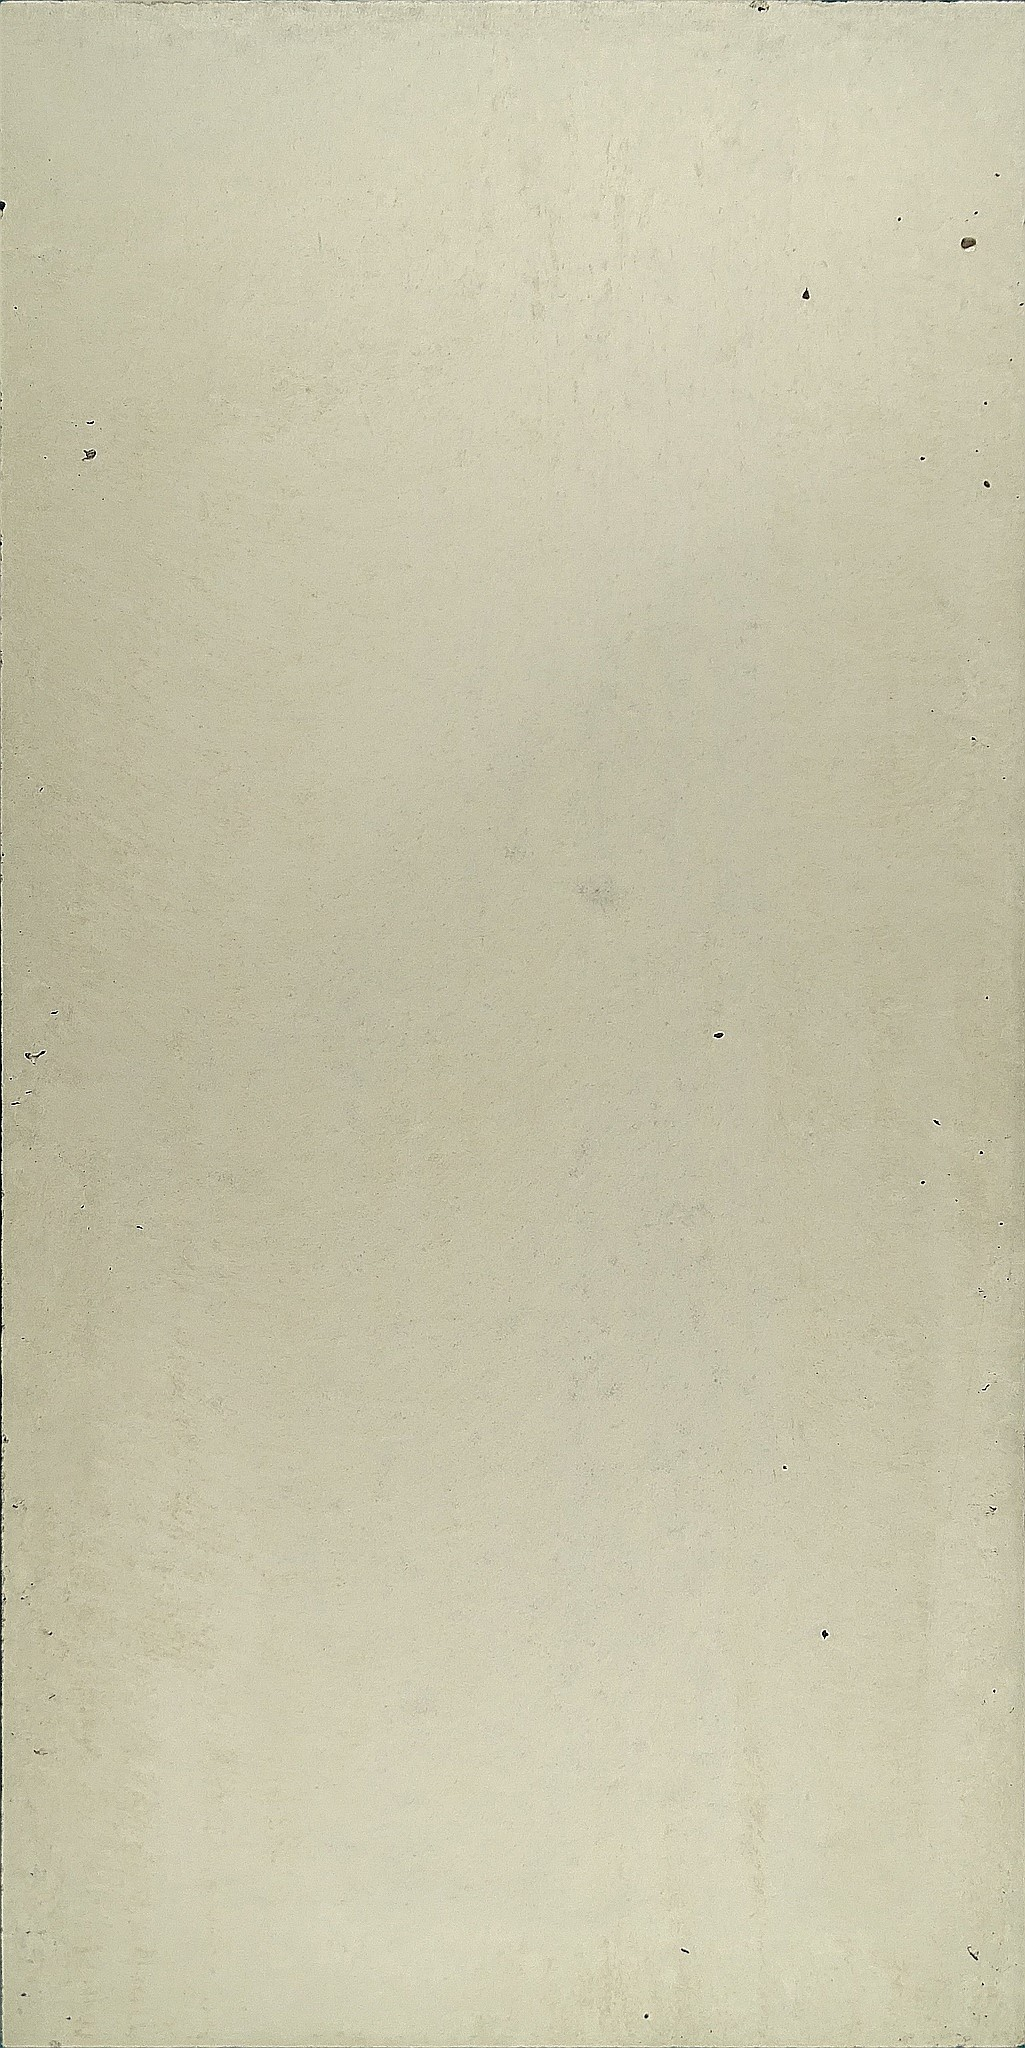
\includegraphics[width=0.2\textwidth]{pictures/BioCast_M2_r_S2.jpg}
		\label{pic:Fehlausleuchtung_a}
	}
	\subfigure[Fehlerhaft ausgeleuchtetes Graustufenbild]{
		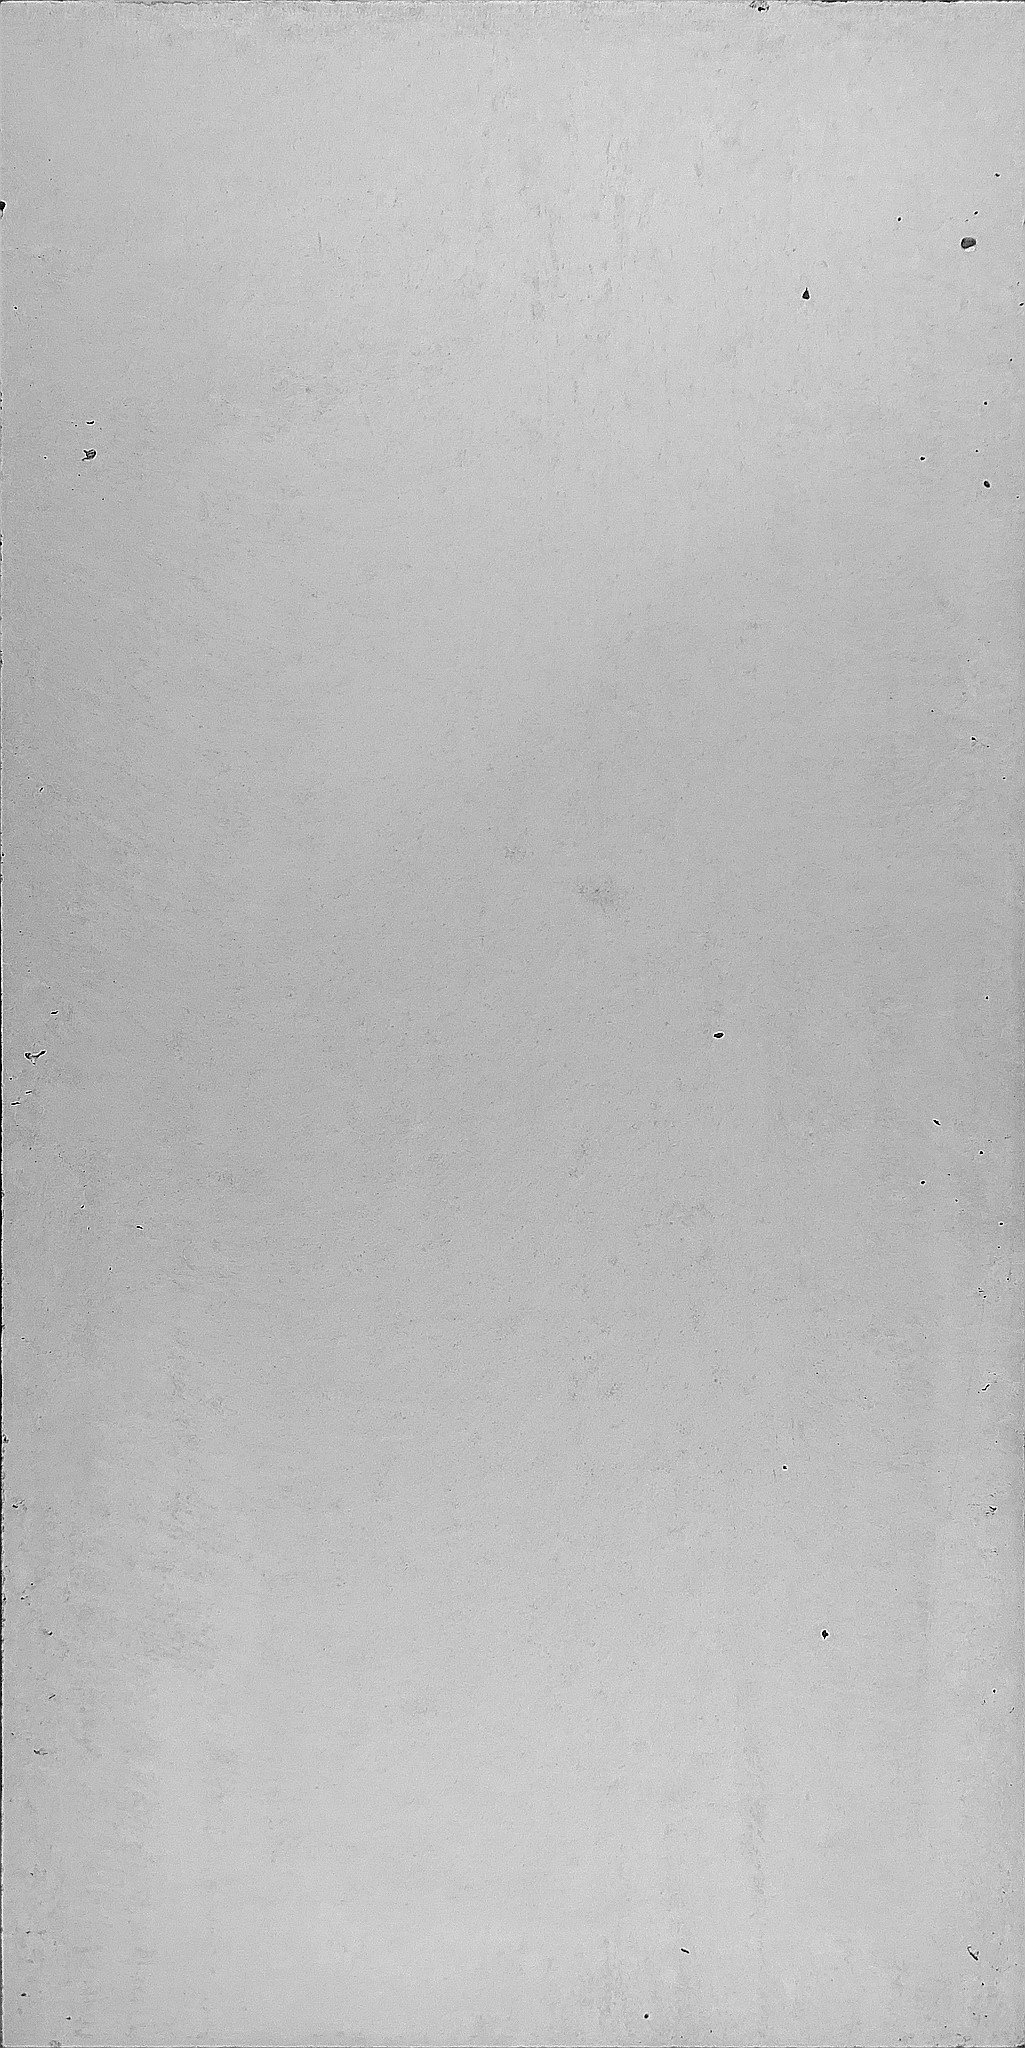
\includegraphics[width=0.2\textwidth]{pictures/BioCast_M2_r_S2_gray.jpg}
		\label{pic:Fehlausleuchtung_b}
	}
	\subfigure[Korrigiertes Graustufenbild]{
		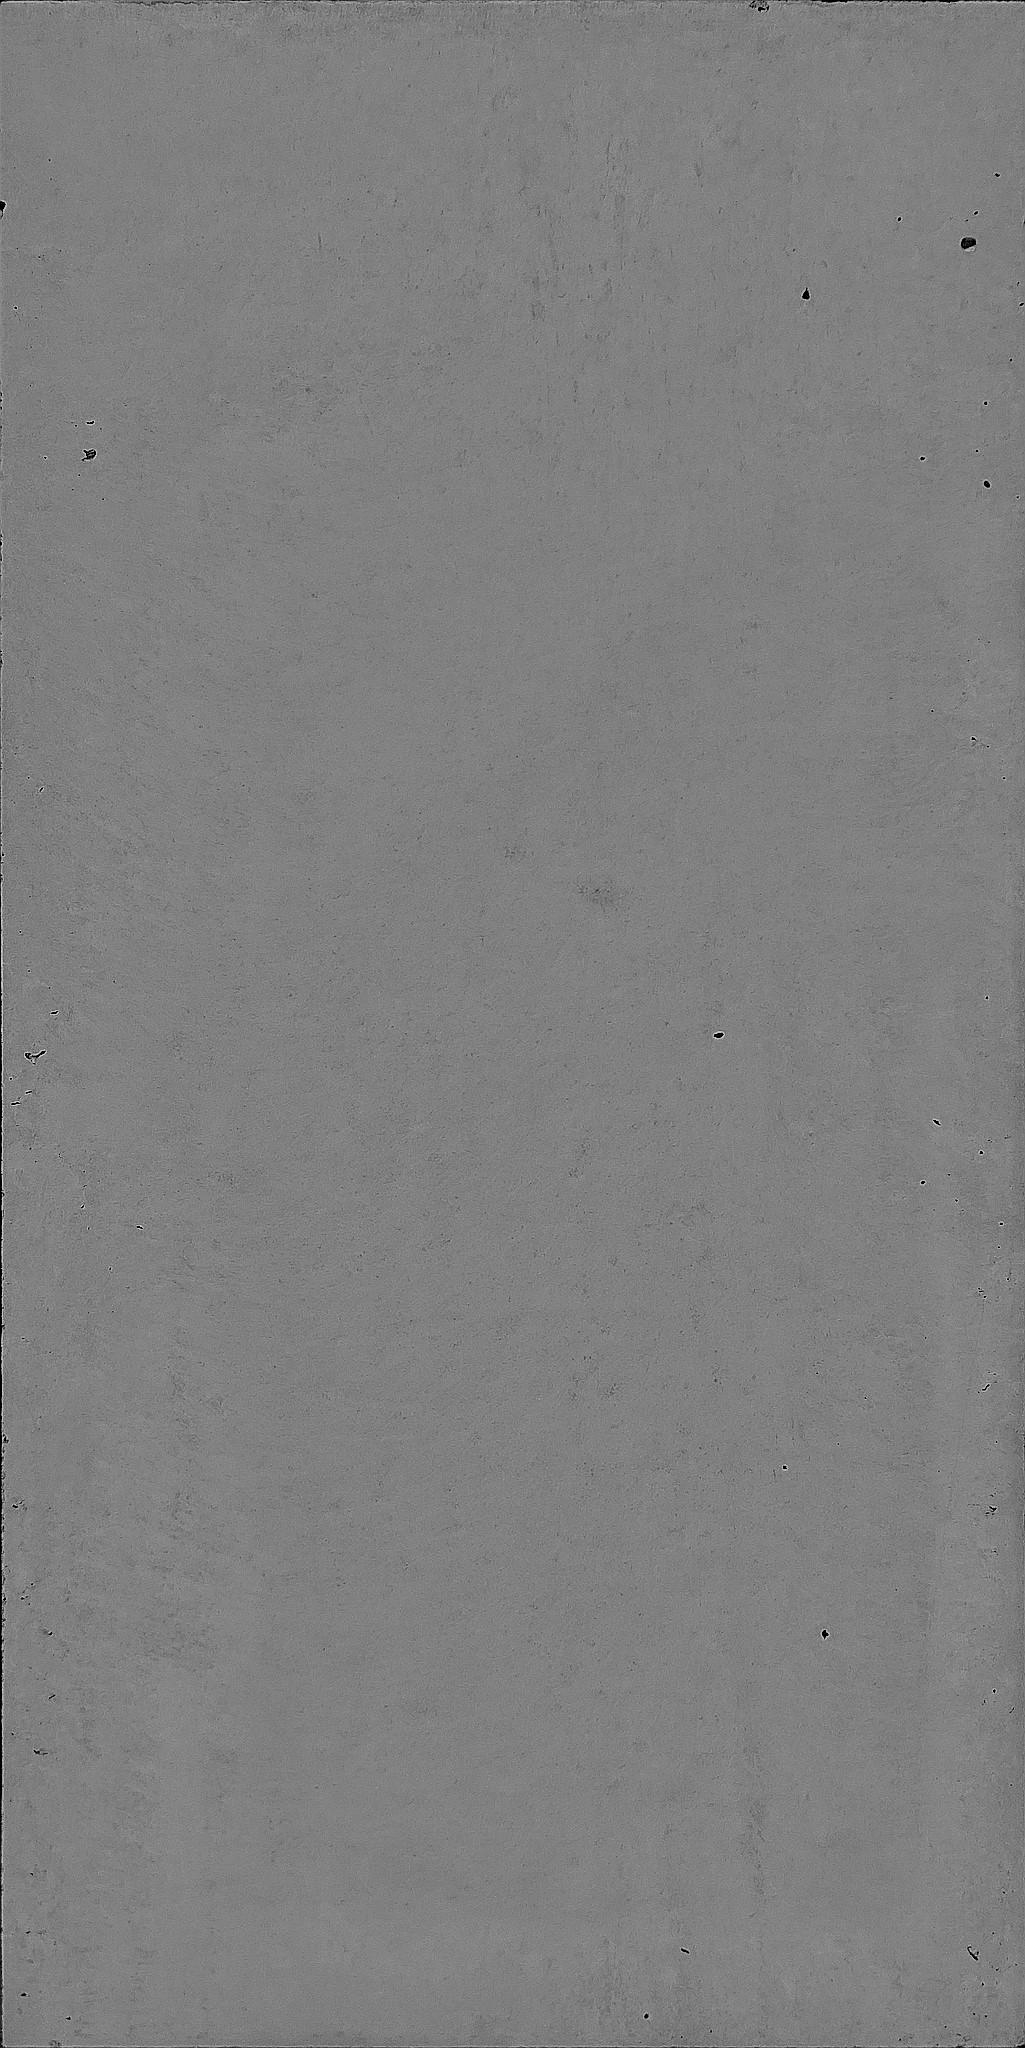
\includegraphics[width=0.2\textwidth]{pictures/BioCast_M2_r_S2_corr.jpg}
		\label{pic:Fehlausleuchtung_c}
	}
	\subfigure[Binarisiertes Bild zur Porenanalyse]{
		
\includegraphics[width=0.2\textwidth,frame]{pictures/BioCast_M2_r_S2_pores.jpg}
		\label{pic:Pores}
	}
	\caption{Bildverarbeitungsschritte}
\end{figure}

\subsection{Ermittlung der Grauwertverteilung in horizontaler und vertikaler Richtung}

Das folgende Verfahren dient hauptsächlich zur Identifikation von inhomogenen Strukturen auf der Oberfläche in $x$ oder $y$-Richtung. 
Die Randbereiche $r = \lfloor 0.03 h \rfloor$ (3\,\% der Bildhöhe $h$) werden von dieser Untersuchung ausgeschlossen.
Im Folgenden wird der Algorithmus anhand der horizontalen Grauwertverteilung beschrieben.
In der horizontalen Richtung wird der mittlere Grauwert $g_{\text{mean}, x}$ der orthogonal dazu verlaufenden Pixel ermittelt (vgl. Gleichung \ref{eq:greyMeanX}) und von dem Durchschnittsgrauwert $g_\text{mean}$ (vgl. Gleichung \ref{eq:greyMean}) des Gesamtbildes abgezogen.

\begin{equation}
	g_{\text{mean}, x} = \frac{ \sum \limits_{y=r+1}^{h-2r} g_{xy} }{h-2r} 
	\label{eq:greyMeanX}
\end{equation}
\begin{equation}
	g_\text{mean} = \frac{ \sum \limits_{x=r+1}^{b-2r} \sum \limits_{y=r+1}^{h-2r} g_{xy} }{(h-2r)(b-2r)}
	\label{eq:greyMean}
\end{equation}
\begin{equation}
	g_{\text{diff}, x} = \left| g_\text{mean} - g_{\text{mean}, x} \right|  
	\label{eq:greyMean}
\end{equation}
Die Absolutwerte der so berechneten Differenz wird anschließend über die gewählte Richtung aufsummiert.
Die Berechnung der horizontalen Grauwertabweichung $g_\text{diff, horizontal}$ ist in Gleichung \ref{eq:greyMeanDiffX} dargestellt.
Um insbesondere eine Aussage über unerwünschte Abweichungen zu treffen, wurde ein Grenzwert von 0.4 für $g_{\text{diff}, x}$ festgelegt.
\begin{equation}
	g_\text{diff, horizontal} = \frac{ \sum \limits_{x=r+1}^{b-r} g_{\text{diff}, x}}{(b-2r)} ~~~ mit ~~~ g_{\text{diff}, x} > 0.4
	\label{eq:greyMeanDiffX}
\end{equation}
Je größer der resultierende Wert, desto größere, inhomogene Helligkeitsabweichungen zeigen sich über die jeweilige Richtung.
Für die dargestellten Parameter ergibt sich bei den untersuchten Proben und den verwendeten Parametern in etwa folgende Einteilung:
\begin{enumerate}
	\item homogene Fläche $<$ 0.3
	\item leichte Strukturen erkennbar 0.3 ... 0.5
	\item deutliche Strukturen erkennbar $>$ 0.5
\end{enumerate}
Unterscheiden sich $g_\text{diff, horizontal}$ und $g_\text{diff, vertical}$ um mehr als 0.1 müsste ein richtungsabhängiges Muster auf der Oberfläche sichtbar sein. 
Negative Auswirkungen auf diese Untersuchung sind durch folgende Einflüsse zu erwarten:
\begin{enumerate}
	\item Fehlerhafter Bildzuschnitt (z.B. schwarze Pixelkante)
	\item Poren
	\item Extrem einseitiger Beleuchtungsfehler
	\item Vergleich von Datensätzen unterschiedlicher Auflösung (Auflösung der Bilder muss normiert werden!)
\end{enumerate}

\begin{figure}[h!]
	\centering
	\subfigure[homogene Oberfläche]{
		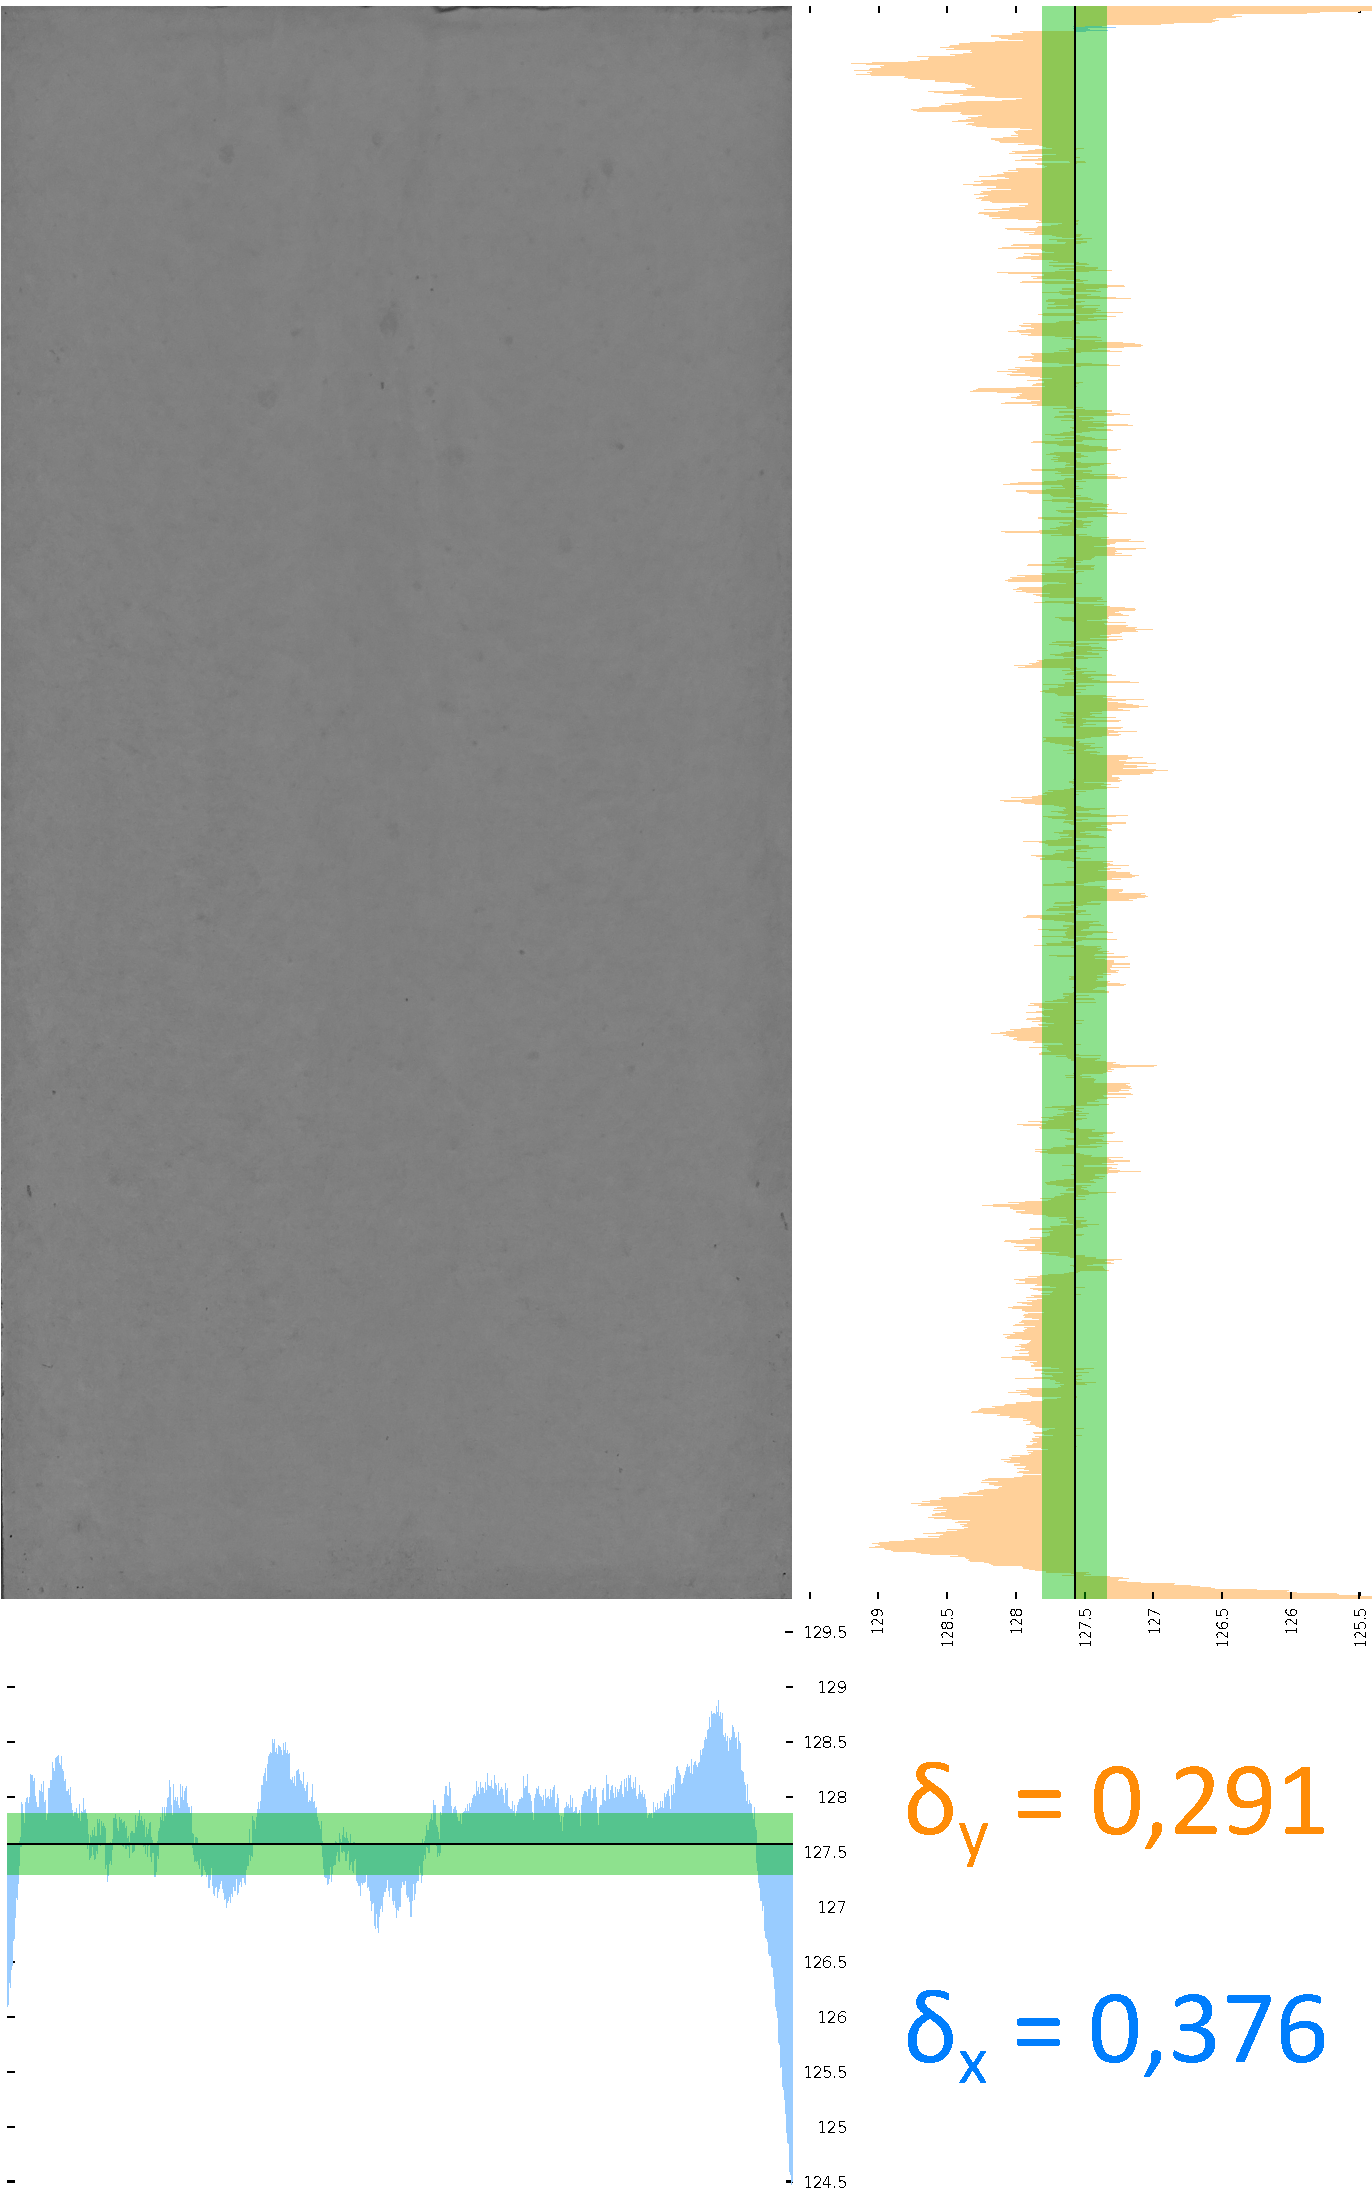
\includegraphics[height=0.45\textheight]{pictures/bspGut.pdf}
		\label{pic:raster}
	}
	\subfigure[inhomogene und strukturierte Oberfläche]{
		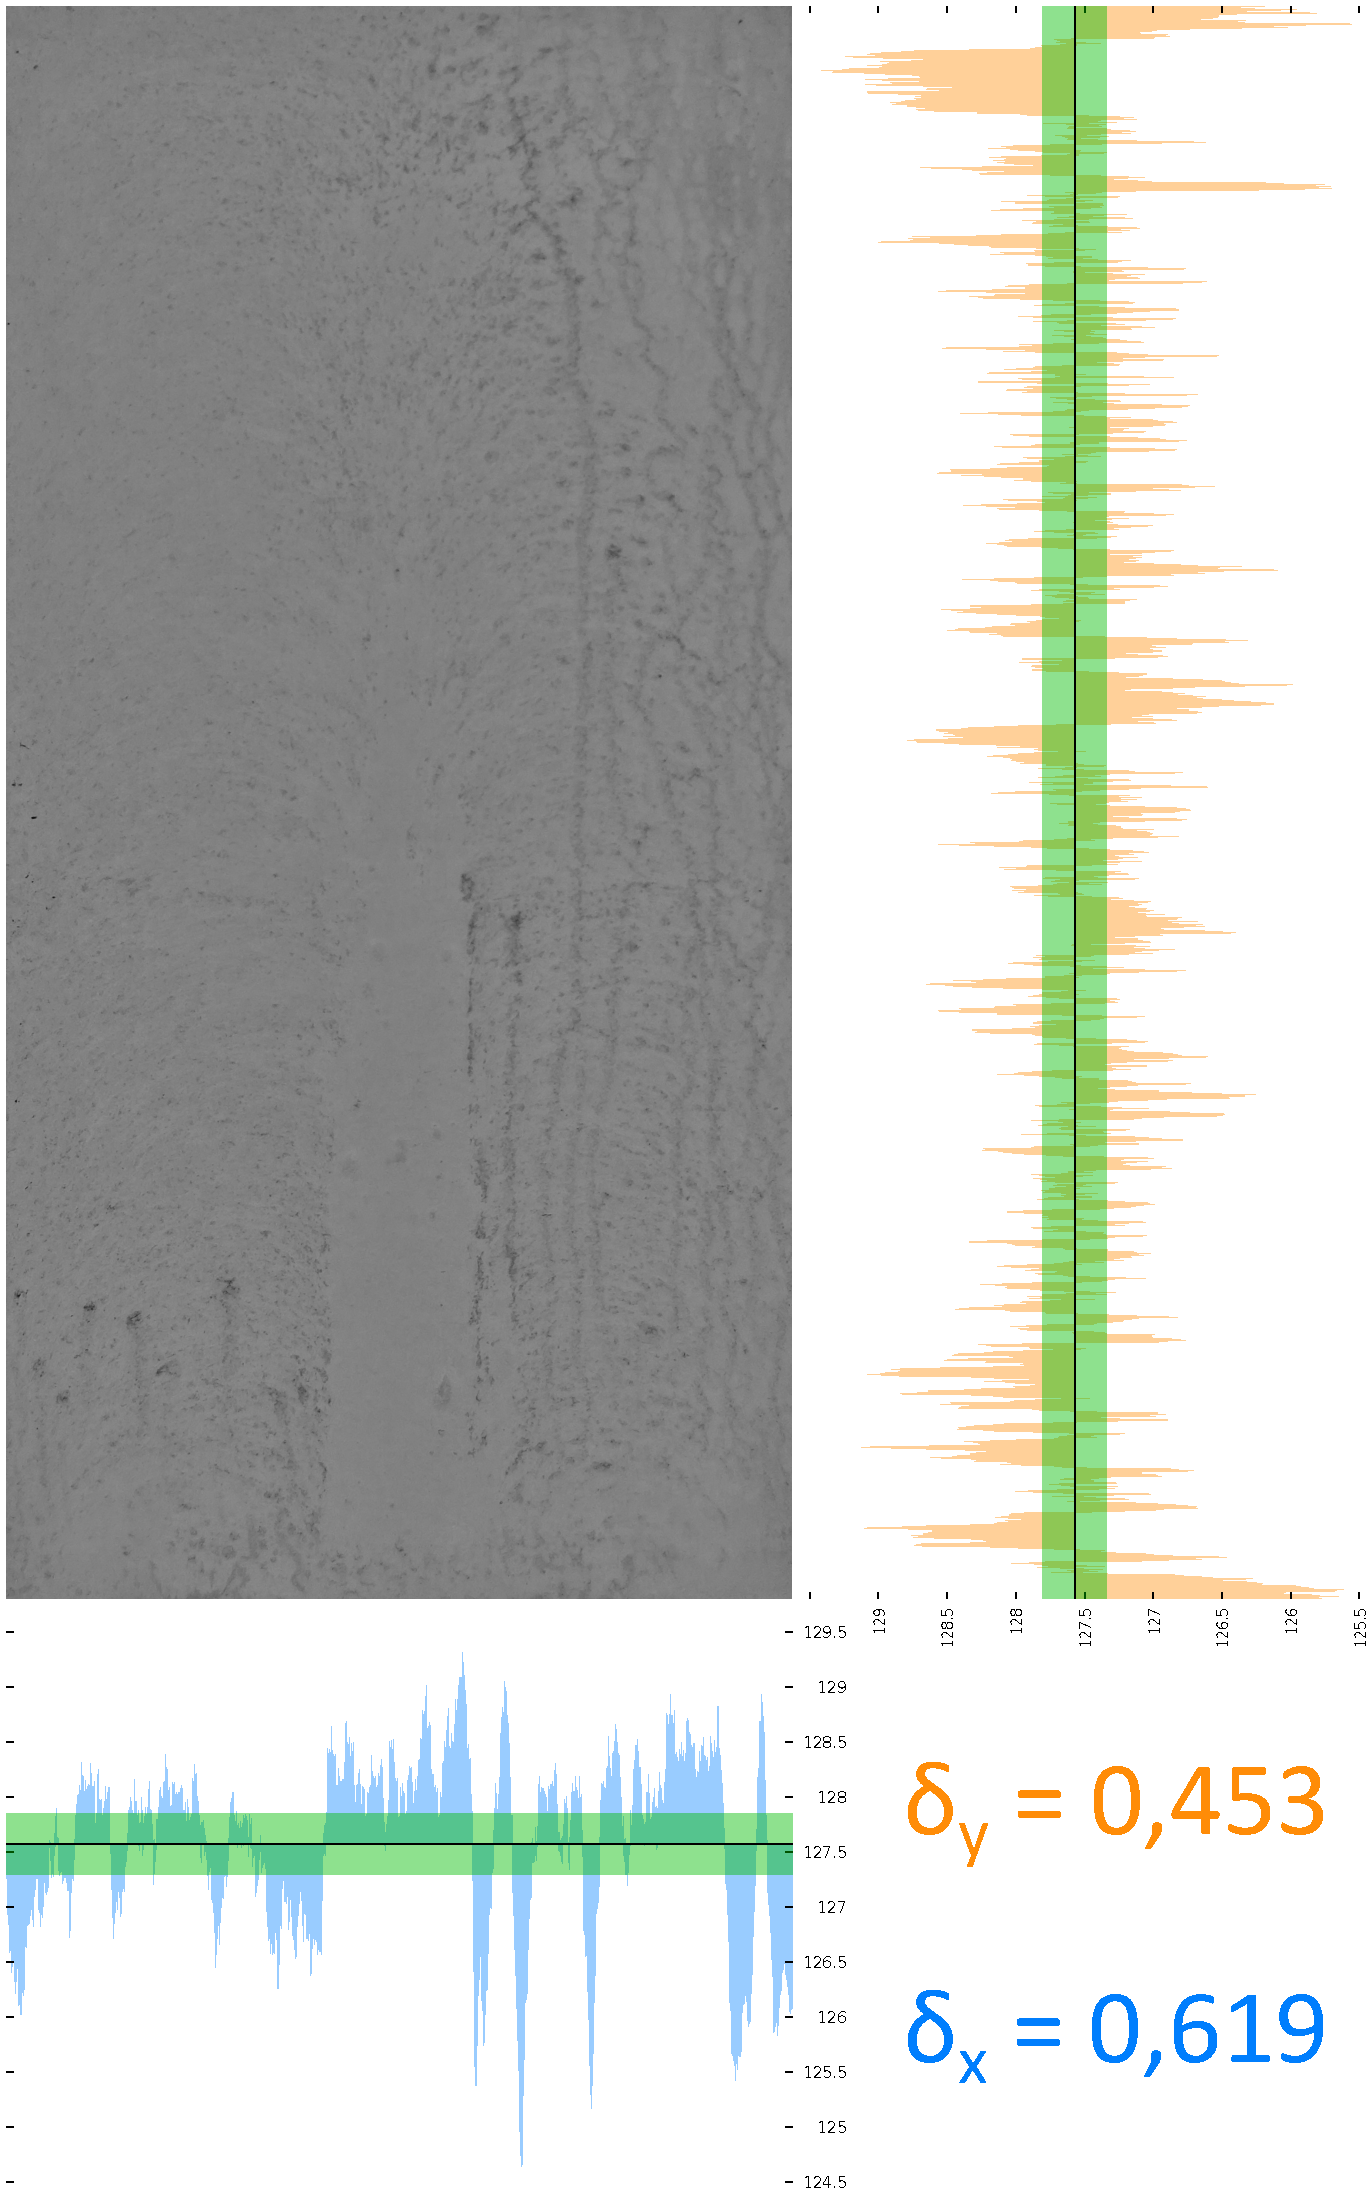
\includegraphics[height=0.45\textheight]{pictures/bspSchlecht.pdf}
		\label{pic:raster_grau}
	}
	\caption{Graphische Darstellung der Analyse der Betonstruktur}
\end{figure}

\subsection{Flächenbasierte Grauwertabweichungen}
\begin{enumerate}
	\item Unterteilung des Bildes in mehrere kleinere Bereiche (Definiert durch die Variablen \textit{rows} und \textit{columns} (Im Folgenden $X$ und $Y$ genannt)  in \textit{start\_process.py} (Abb. \ref{pic:raster})
	\item Berechnung des durchschnittlichen Grauwertes $g$ und der Standardabweichung der Grauwerte $\sigma_g$ innerhalb des Bereiches (Abb. \ref{pic:raster_grau})
	\item In \textit{start\_process.py} werden Grauwertabweichungen der Nachbarbereiche $\delta N$ ermittelt (Abb. \ref{pic:raster_delta_n})
	\item Das Bild aus Punkt 4 wird über einen Helligkeitsgrenzwert von 51 (im Wertebereich 0 \dots 255) binarisiert, um die Porenfläche zu ermitteln (Abb. \ref{pic:Pores})
	\item Abschließend werden die ermittelten Werte ausgewertet, indem Mittelwerte und Standardabweichungen ($\bar{g}$, $\bar{\sigma}_g$, $\sigma_{\delta N}$, $\bar{\sigma}_{\delta N}$) der genannten Paramertern berechnet werden
\end{enumerate}

\begin{figure}[h!]
	\centering
	\subfigure[Unterteilung]{
		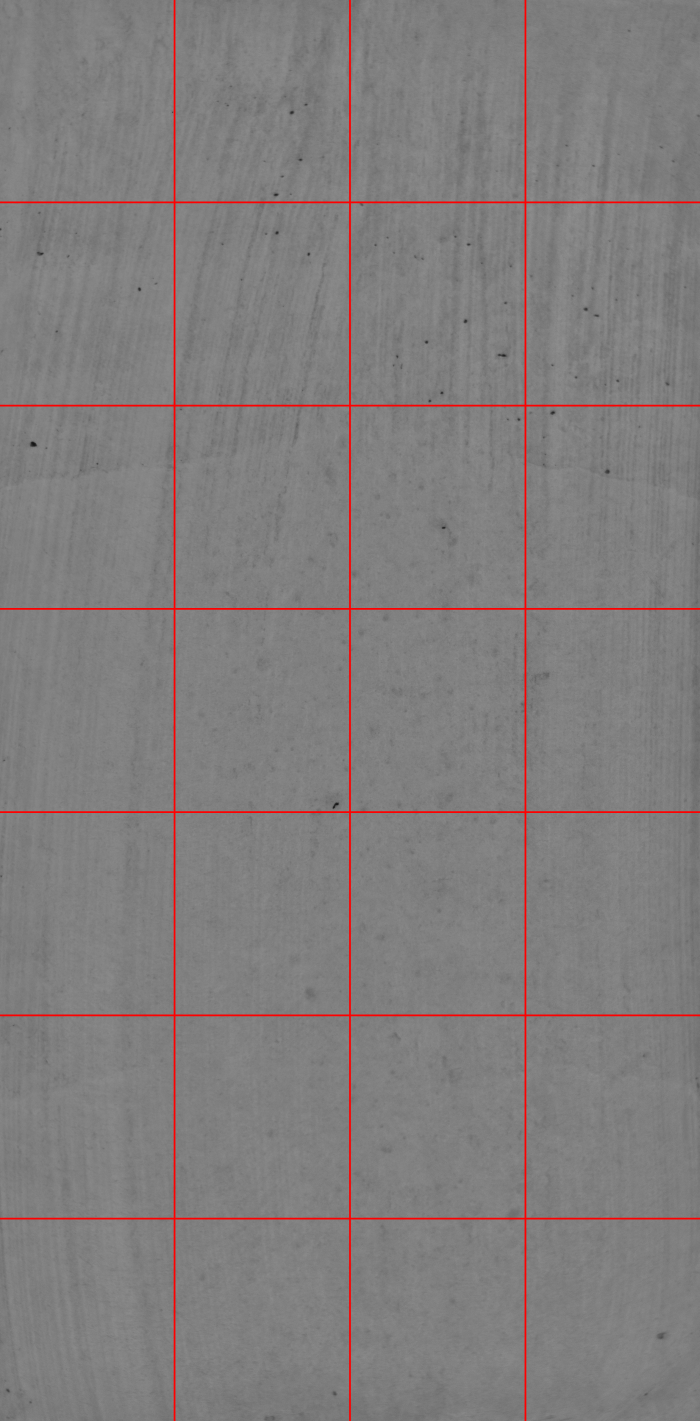
\includegraphics[height=0.3\textheight]{pictures/Raster.png}
		\label{pic:raster}
	}
	\subfigure[Bestimmung durchschnittlicher Grauwerte]{
		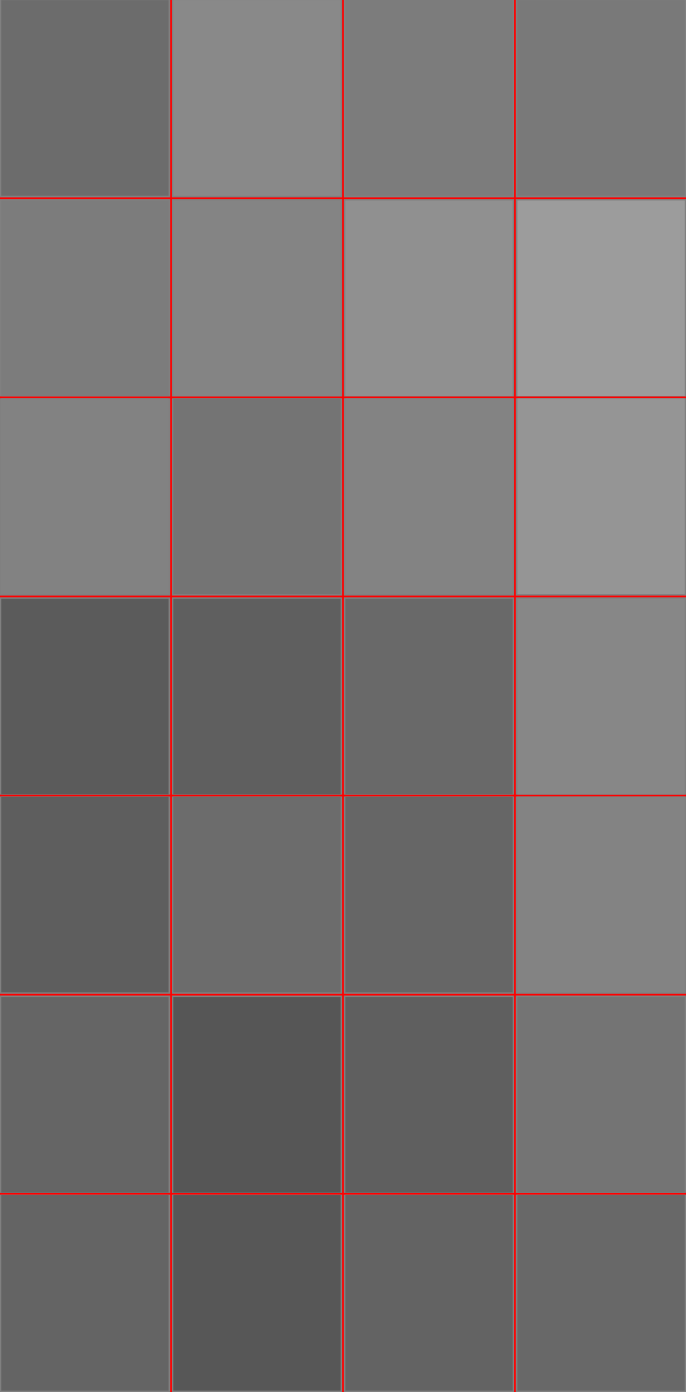
\includegraphics[height=0.3\textheight]{pictures/Raster_grau.png}
		\label{pic:raster_grau}
	}
	\subfigure[Bestimmung der Grauwertabweichungen der Nachbarbereiche]{
		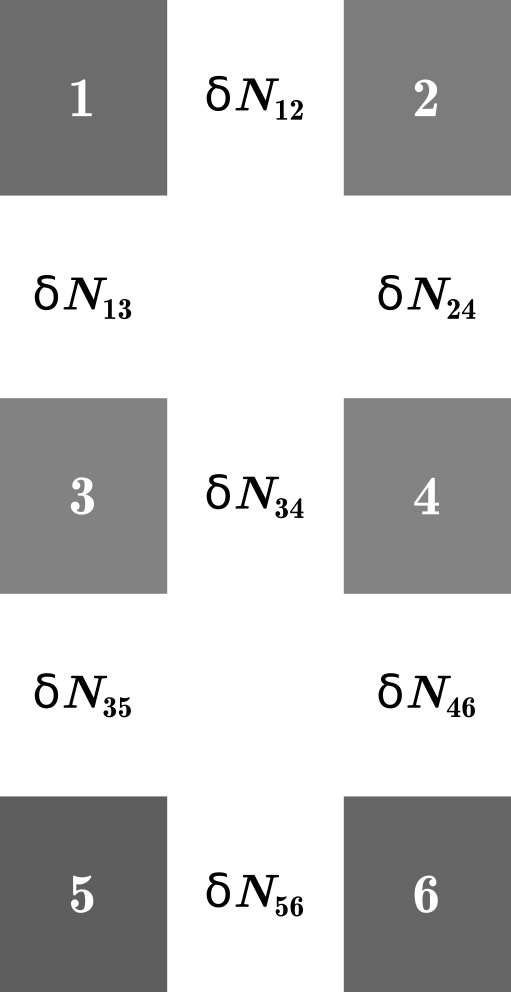
\includegraphics[height=0.3\textheight]{pictures/Raster_delta_n.png}
		\label{pic:raster_delta_n}
	}
	\caption{Bildunterteilung zur Bestimmung der Grauwertabweichungen}
\end{figure}


\FloatBarrier

\section{Bildaquirierung}
\subsection{Probekörper}
Das Merkblatt \textit{Sichtbeton} des \textsc{Deutschen Beton- und Bautechnik Vereins e.V.} schreibt zur Beurteilung der Sichtbetonqualität eine Fläche von 50 $\times$ 50\,cm vor. Dieses Programm ist hingegen auf die Auswertung von Flächen von 25 $\times$ 50\,cm ausgelegt, kann jedoch auch die geforderten 500\,cm$^2$ verarbeiten.

\subsection{Ausleuchtung}.

Eine Serie von Probekörpern oder Probeflächen sollte unter möglichst identischen und gleichmäßigen Beleuchtungsverhältnissen fotografiert werden. Ausleuchtungsfehler, wie in Abbildung \ref{pic:Fehlausleuchtung_a} dargestellt, kann allerdings problemlos durch ausgeglichen werden (vgl Abb. \ref{pic:Fehlausleuchtung_c}).

\subsection{Bildaufnahme}

Die Bilder einer Probenserie müssen bei identischen Bedigungen aufgenommen werden. Darunter fällt eine möglichst gleichmäßige Ausleuchtung sowie identische Kameraeinstellungen.
Für eine Porenanalyse ist streifender Lichteinfall über die Betonoberfläche sinnvoll, da orthogonal auftreffendes Licht Poren ausleuchten kann und damit die Erkennung derselben erschwert.

Um Aussagen über die Farbigkeit der Oberflächen treffen zu können, muss die Kamera kalibriert werden. Dies kann mit einer handelsüblichen Farbkalibrationskarte (z. B. Colochecker Passport von Xrite) realisiert werden. Weiterhin müssen die Aufnahmen als Rohdaten und nicht als jpg gespeichert werden, um die Farbkorrektur möglichst verlustfrei durchführen zu können.
An der Professur Bauchemie und Polymere Werkstoffe steht  ein Fotostand (vgl. Abbildung \ref{pic:fotostand}) zur Verfügung.


\begin{figure}[htbp]
	\centering
	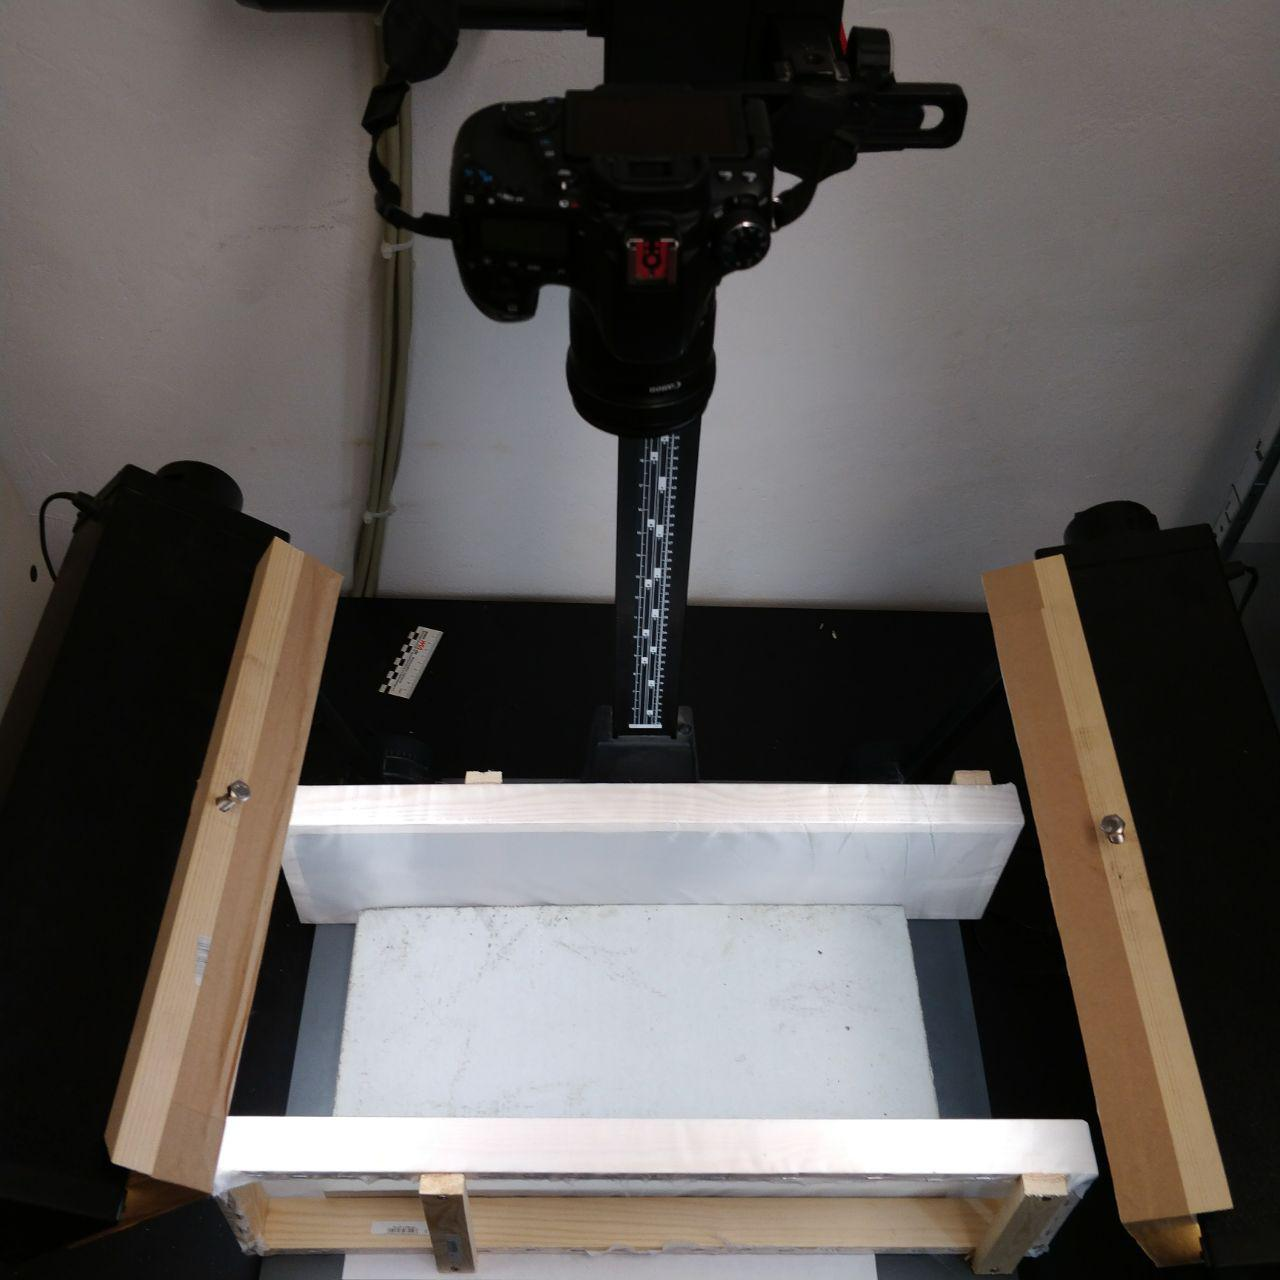
\includegraphics[height=0.4\textheight]{pictures/Fotostand.jpg}
	\caption{Fotostand mit 25 $\times$ 50\,cm Probekörper}
	\label{pic:fotostand}
\end{figure}

Die Kameraeinstellungen müssen bei allen Aufnahmen konstant gehalten werden. Die an der Professur eingesetzte Kamera \textit{SONY SDC-HX400V} wurde beispielsweise mit den folgenden Aufnahmeeinstellungen betrieben:

\begin{itemize} 
	\item ISO-80 
	\item Blende $f$/8 
	\item Belichtungszeit 1/6\,s
	\item Brennweite 7\,mm
\end{itemize}


Die am Stativ des Fotostandes montierte Kamera muss möglichst orthogonal zur Probekörperoberfläche ausgerichtet werden. Bei der Aufnahme sollte darauf geachtet werden, dass die Kamera im Verlauf größerer Probenserien möglichst nicht bewegt wird. Weiterhin sollten die unterschiedlichen Probekörper identisch ausgerichtet werden. Dies lässt sich am einfachsten über einen Anschlag realisieren.

Für die Baustelle wurde ein handelsüblicher mobiler Fotostand umfunktioniert, um eine gleichbleibende Ausleuchtung der Betonoberfläche ermöglichen zu können (Abbildung \ref{pic:Fotobox}). Dieser würfelförmige Fotostand (Kantenlänge $\geq$\,70\,cm) ist umseitig geschlossen, bietet jedoch oberseitig eine Öffnung für eine Kamera. Auf der Seite der Kameraöffnung ist eine LED-Beleuchtung integriert, die eine gleichmäßige, orthogonale Ausleuchtung ermöglicht.

\begin{figure}[htbp]
	\centering
	\subfigure[Bild innerhalb der Fotobox]{
		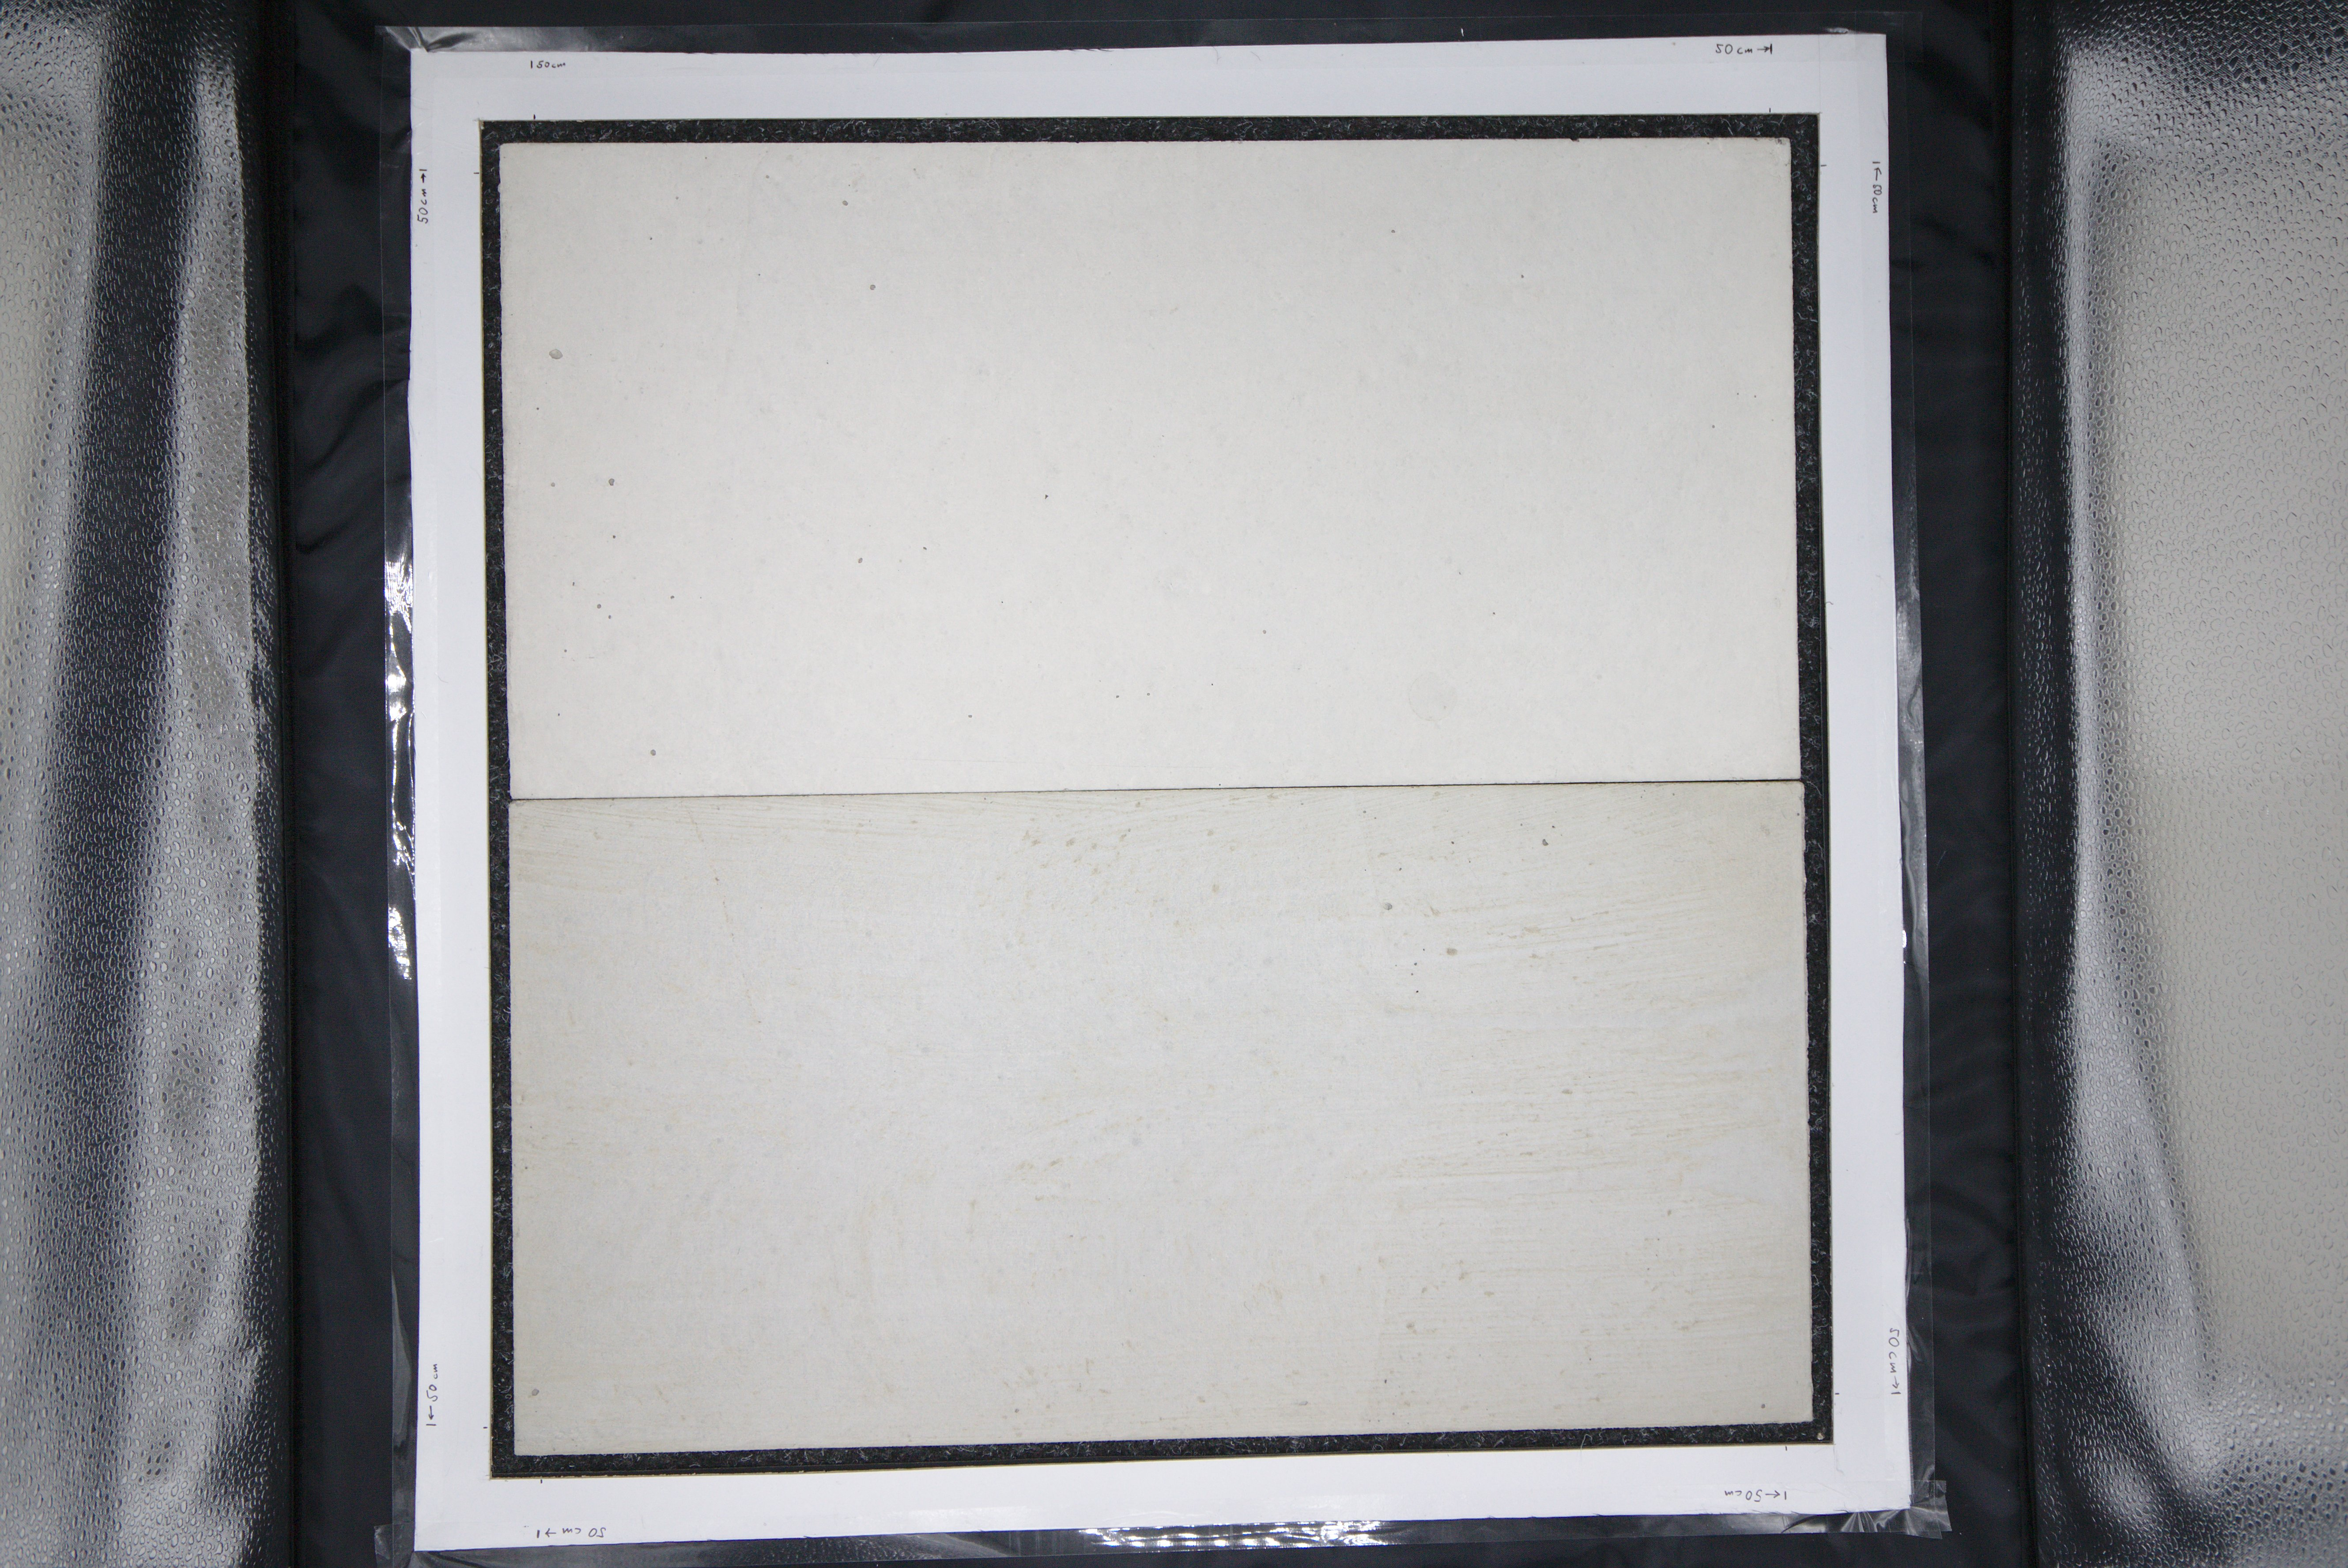
\includegraphics[width=0.45\textwidth]{pictures/Fotobox.jpg}
		\label{pic:Fotobox}
	}
	\subfigure[Farbkalibrationskarte]{
		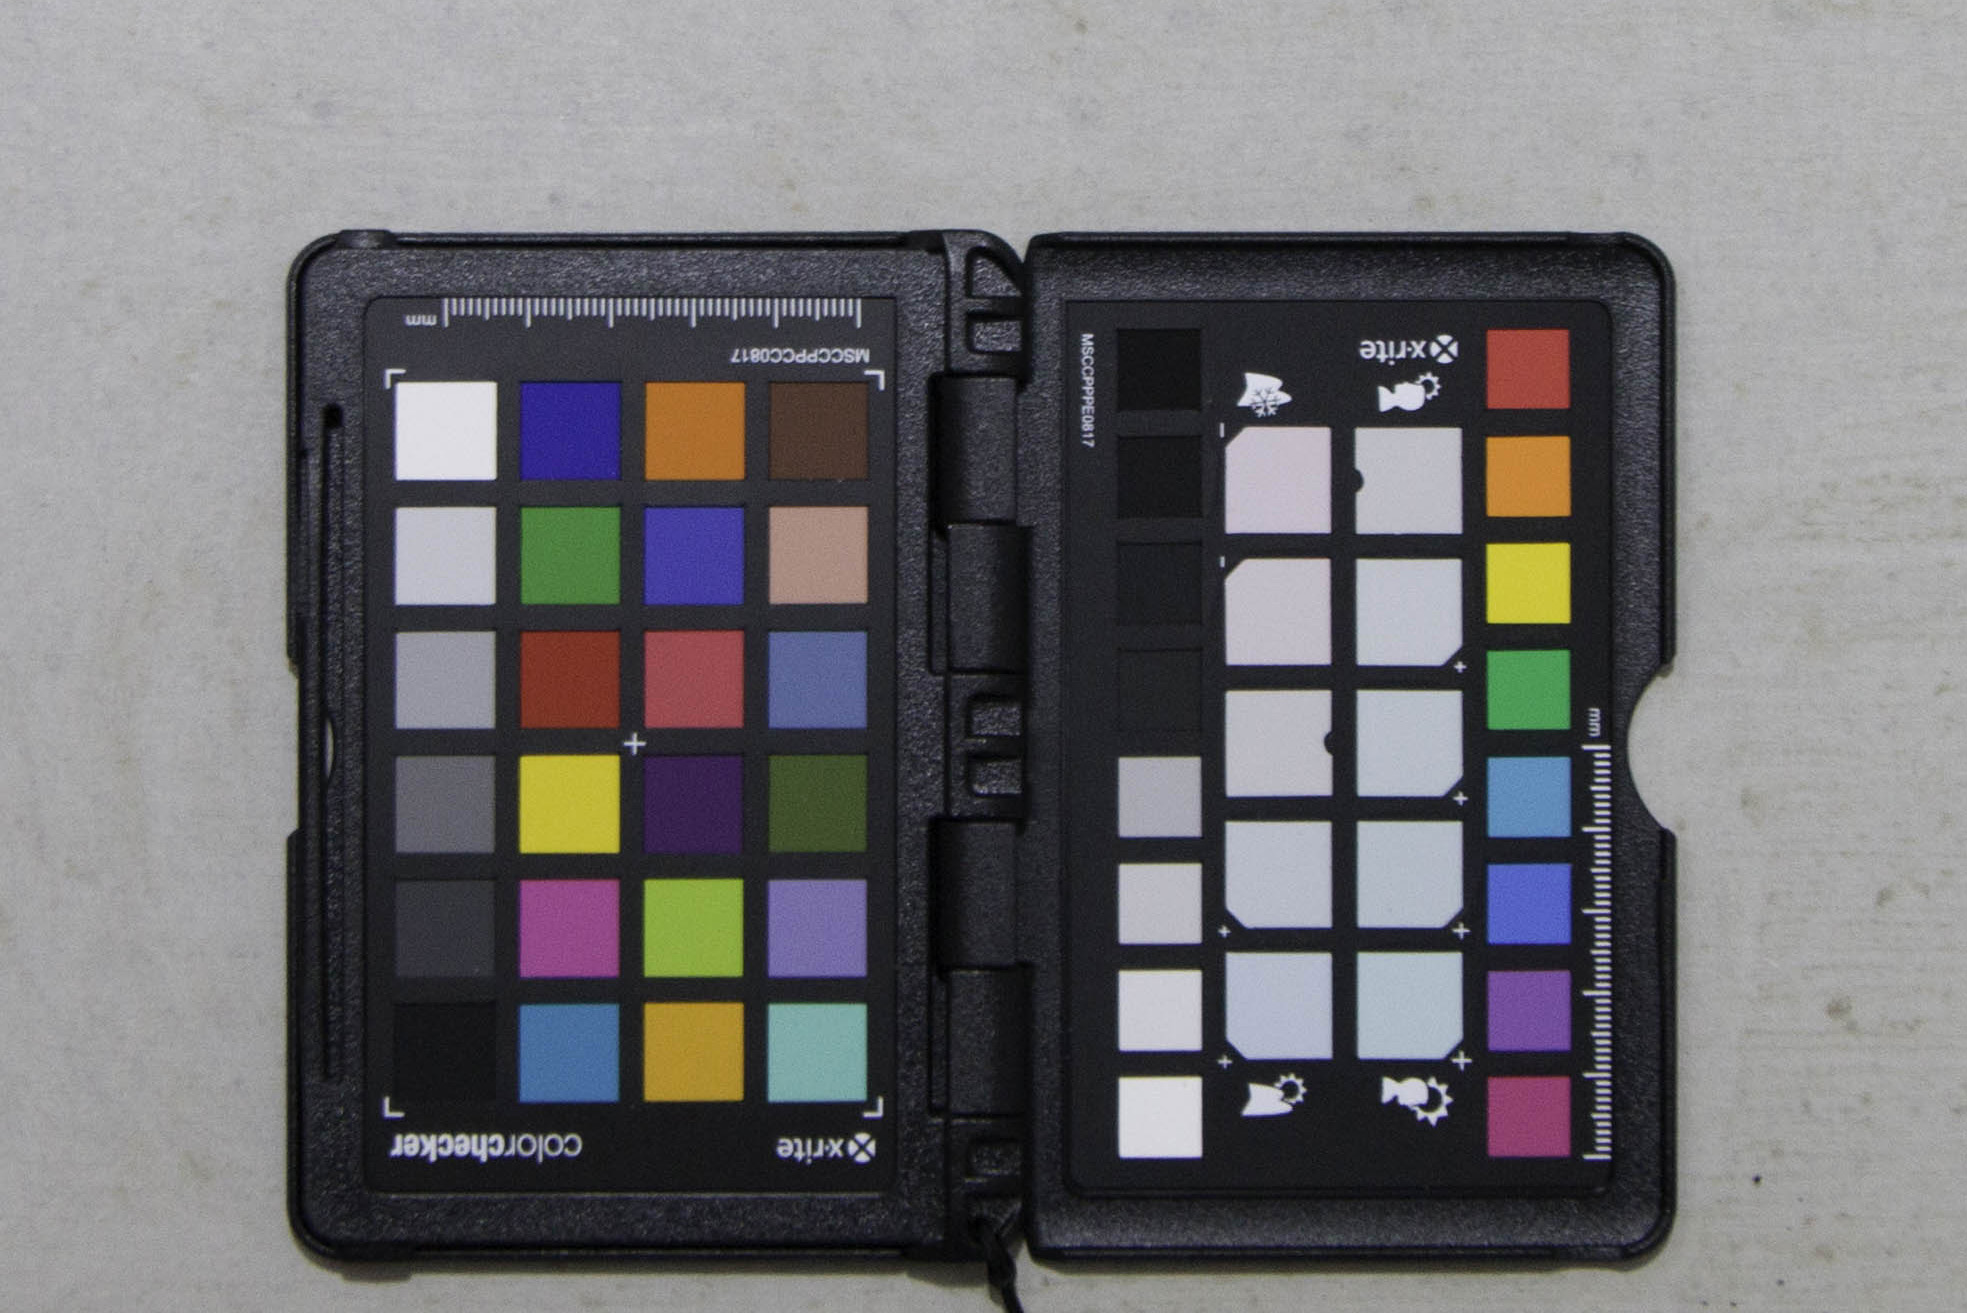
\includegraphics[width=0.45\textwidth]{pictures/colochecker.jpg}
		\label{pic:colorchecker}
	}
	\caption{Bildvorverarbeitungsschritte}
\end{figure}

Der Fotostand wurde so modifiziert, dass gegenüberliegend der Kameraöffnung eine Fläche von ca. 60 $\times$ 60\,cm der Betonoberfläche sichtbar ist. Weiterhin wurden seitlich LED-Leisten angebracht, die einen streifenden Lichteinfall für die Porenanalyse ermöglichen.

Weiterhin wurde ein Standfuß erstellt, mit dem der mobile Fotostand auf verschiedene Höhen eingestellt werden kann.

\subsection{Bildvorbereitung}

Das aufgenommene Bild (Abb. \ref{pic:source}) muss vor der Auswertung vorverarbeitet werden. Darunter zählt der Weißabgleich (Abb. \ref{pic:white}), der über die Farbkalibrationskarte (Abb. \ref{pic:colorchecker}) erfolgt. Weiterhin sollte, wenn möglich eine Objektivkorrektur durchgeführt werden. Abschließend folgt der Zuschnitt auf die Betonfläche (Abb. \ref{pic:cut}).

\begin{figure}[htbp]
	\centering
	\subfigure[Rohdatenbild]{
		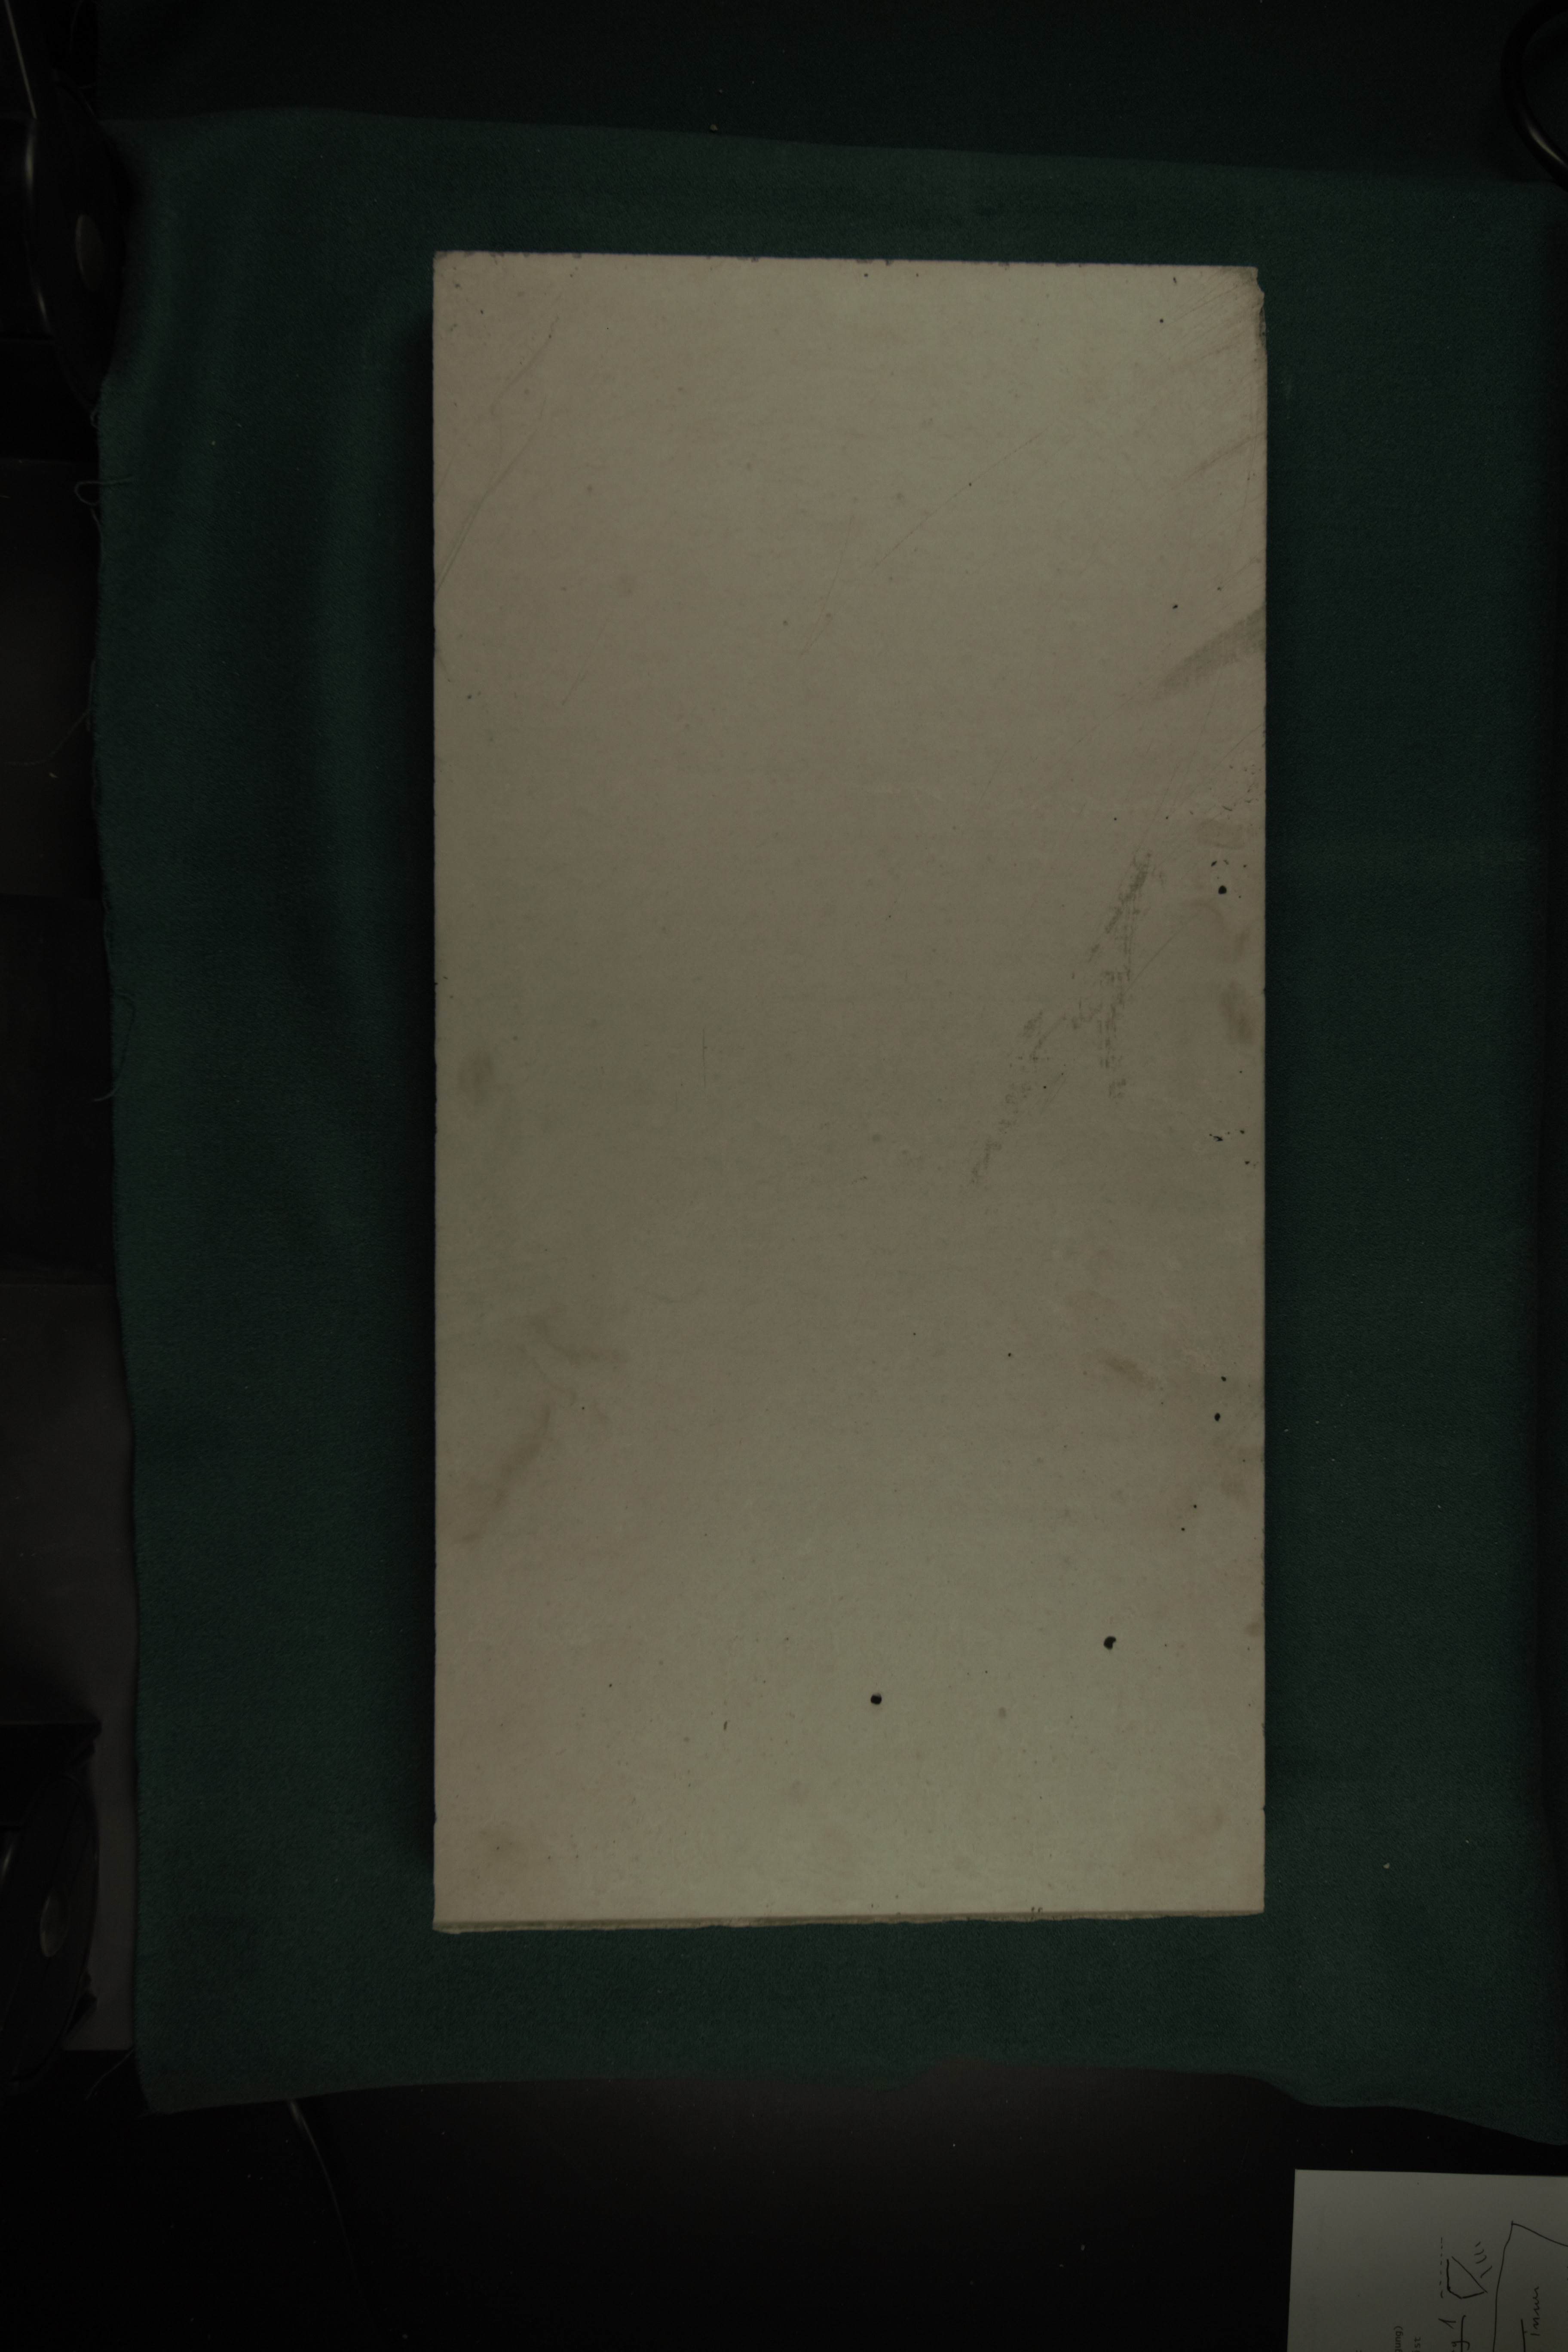
\includegraphics[width=0.3\textwidth]{pictures/source.jpg}
		\label{pic:source}
	}
	\subfigure[Weißabgleich und Aufhellung]{
		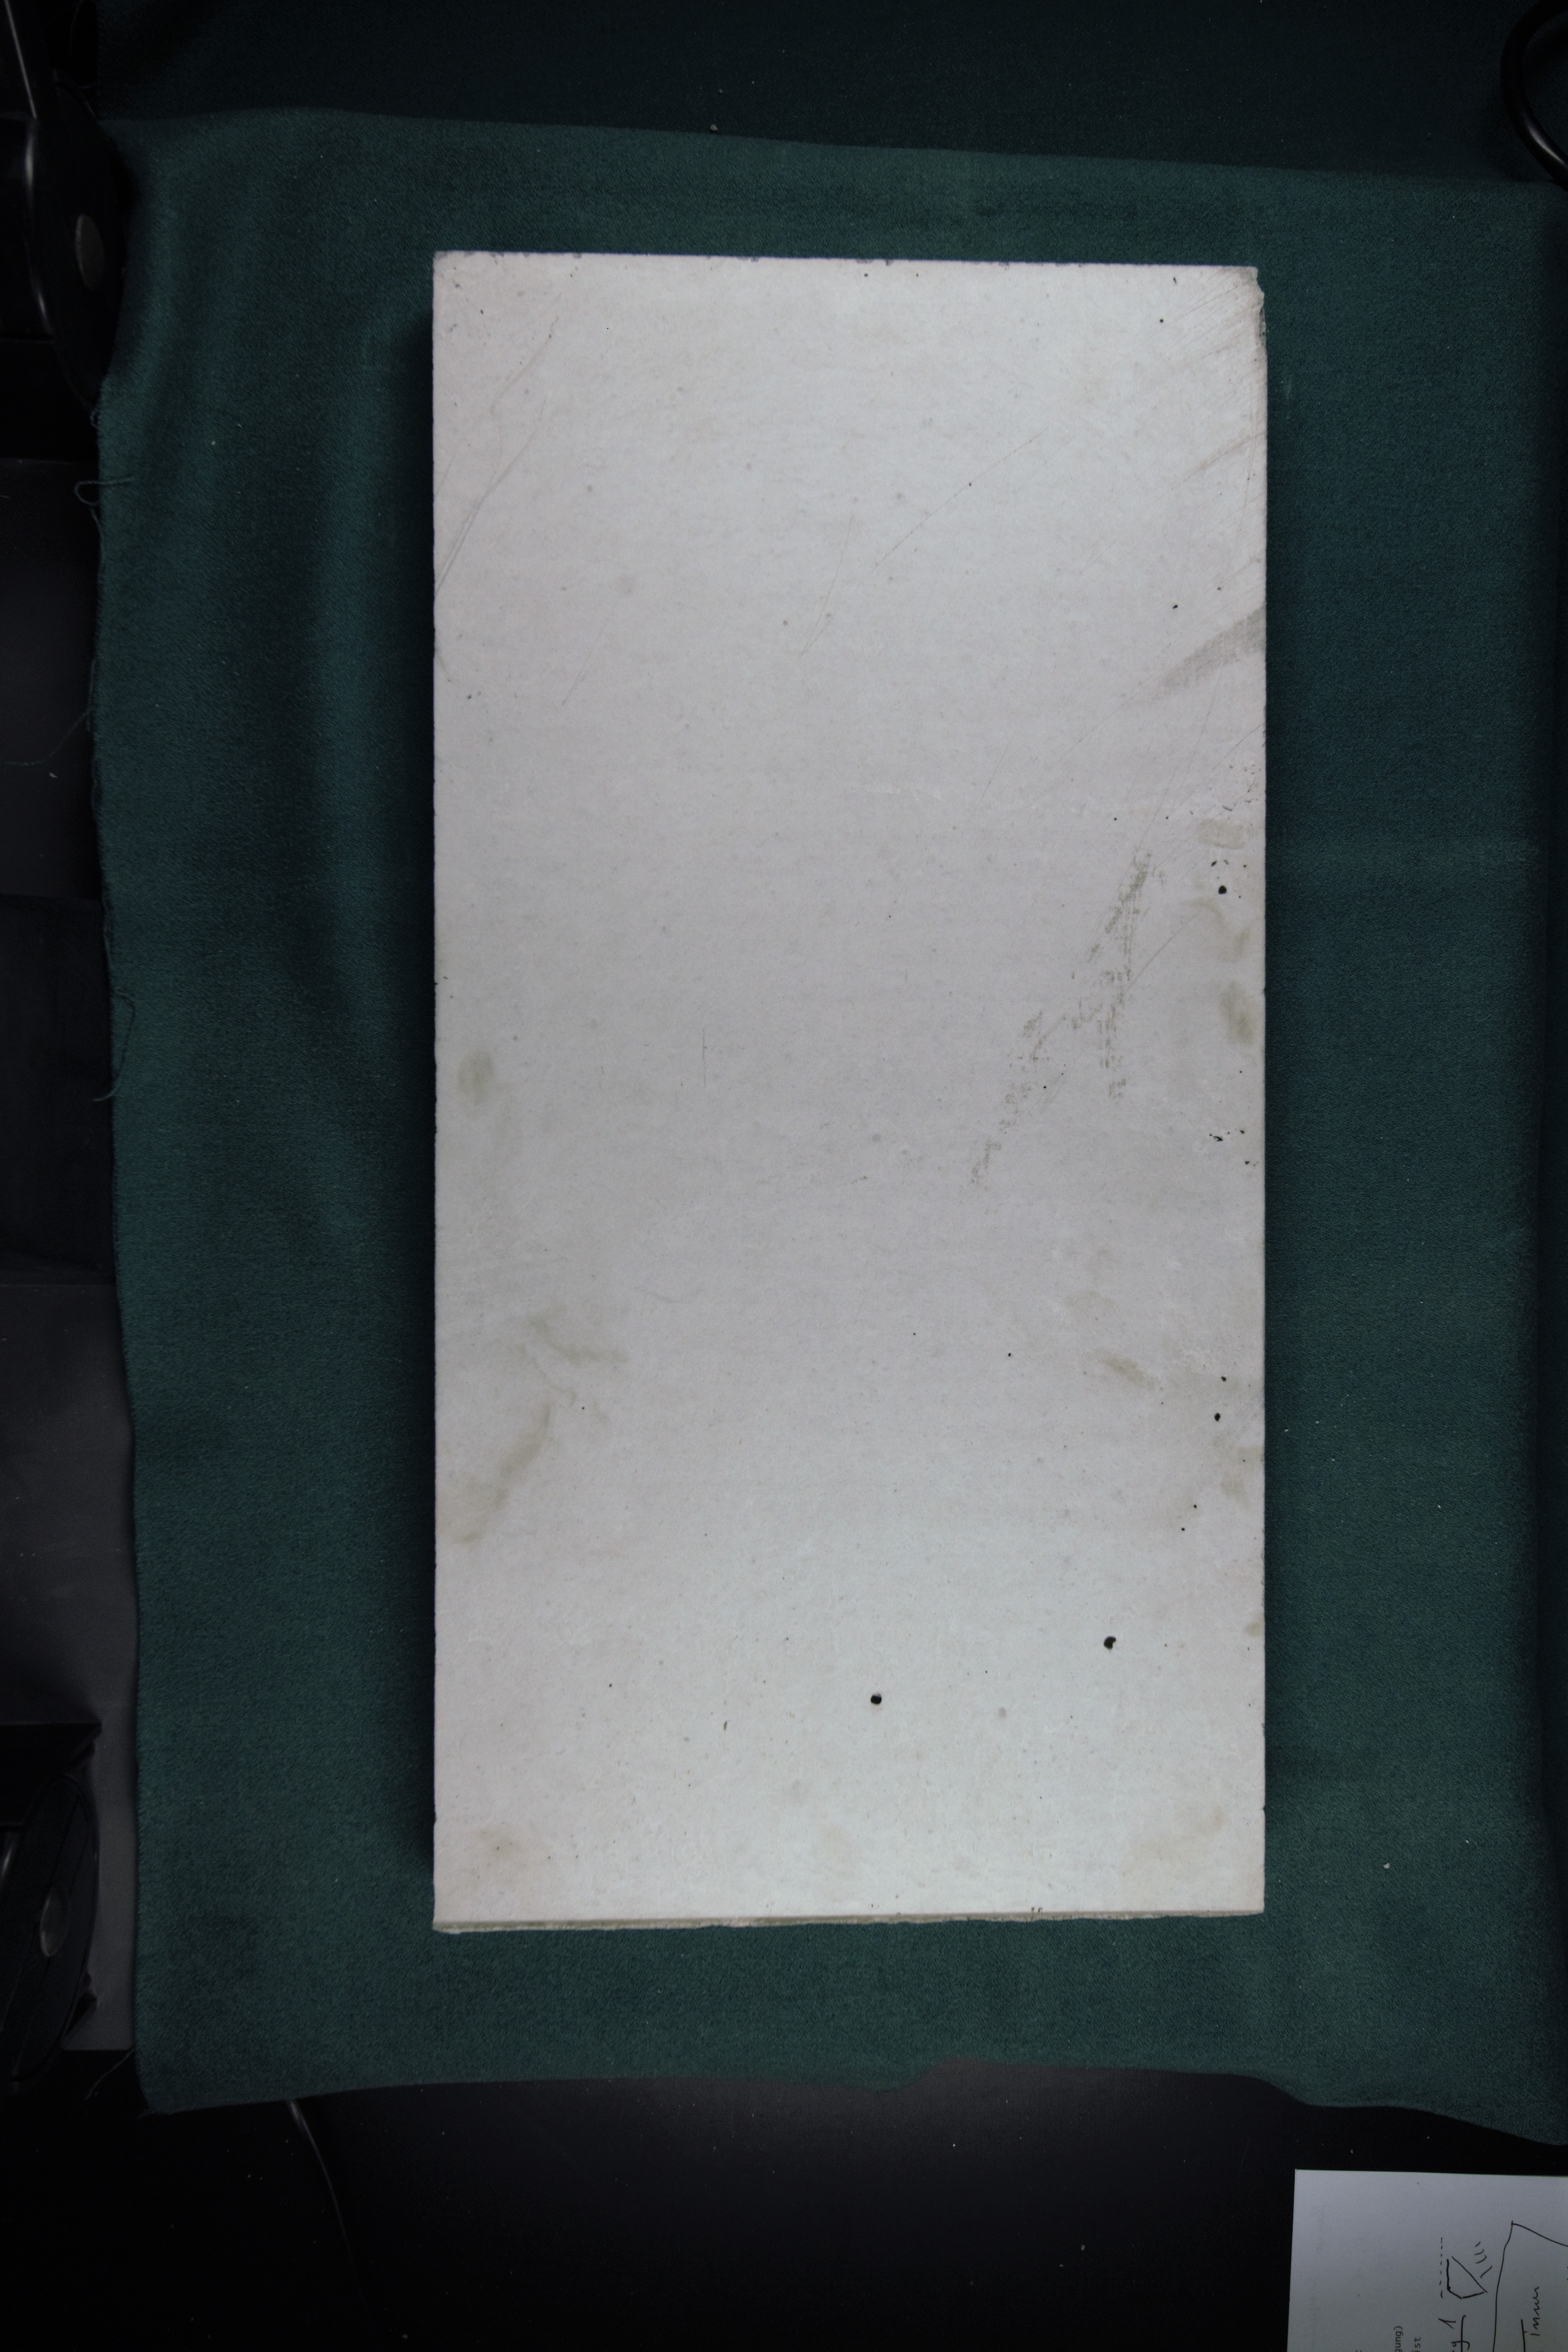
\includegraphics[width=0.3\textwidth]{pictures/white.jpg}
		\label{pic:white}
	}
	\subfigure[Zuschnitt]{
		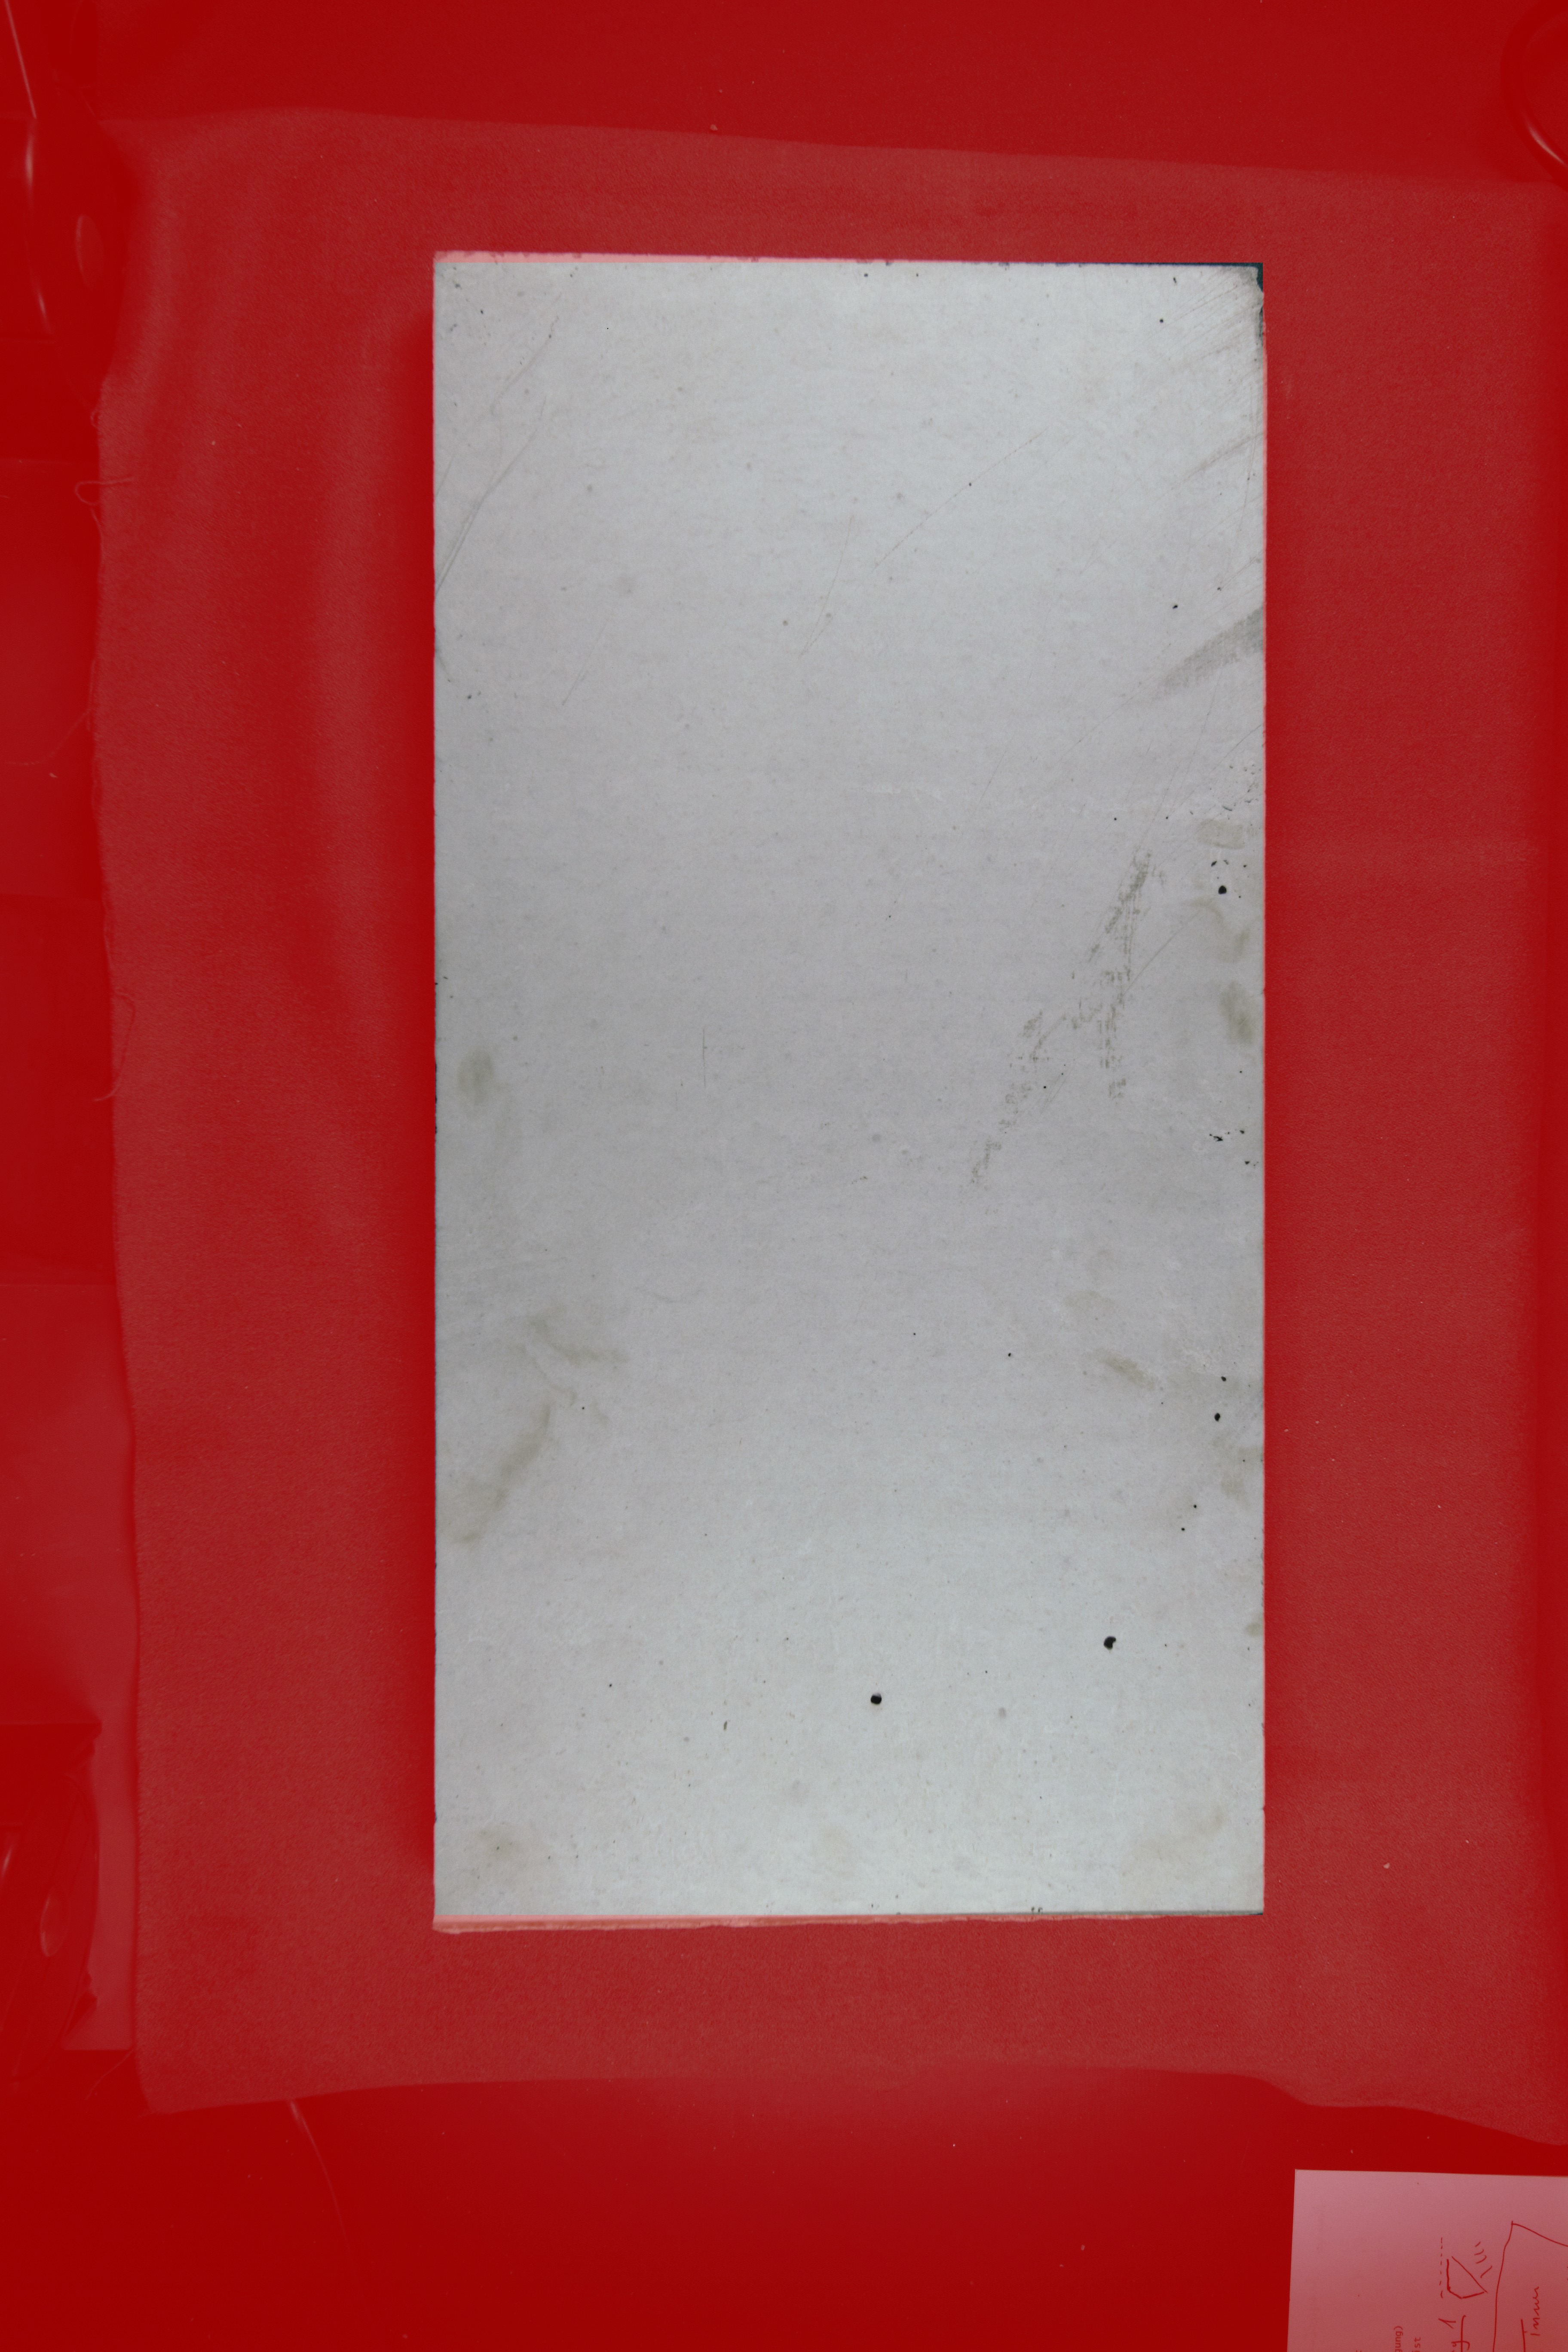
\includegraphics[width=0.3\textwidth]{pictures/cut.jpg}
		\label{pic:cut}
	}
	\caption{Bildvorverarbeitungsschritte}
\end{figure}

Mit Hilfe von \textsc{Darktable} oder \textsc{Lightroom} lassen sich diese Prozesse leicht auf viele Bilder anwenden, nachdem ein Beispielbild entsprechend bearbeitet wurde.

In \textsc{Darktable} werden die Bilder im Bereich \textit{Dunkelkammer} nachbearbeitet. Die Einstellungen können anschließend im Bereich \textit{Leuchttisch} synchronisiert werden (Abb. \ref{pic:darktable}). Dafür muss das bearbeitete Bild markiert sein und unter \textit{Verlaufsstapel} die Schaltfläche \textit{alles kopieren} gedrückt werden. Abschließend werden alle noch zu bearbeitenden Bilder ausgewählt und es wird die Schaltfläche \textit{alles kopieren} gedrückt.

Über \textit{ausgewählte exportieren} lassen sich die Bilder nun in einem neuen Ordner abspeichern und mit dem Script bearbeiten.

\begin{figure}[htbp]
	\centering
	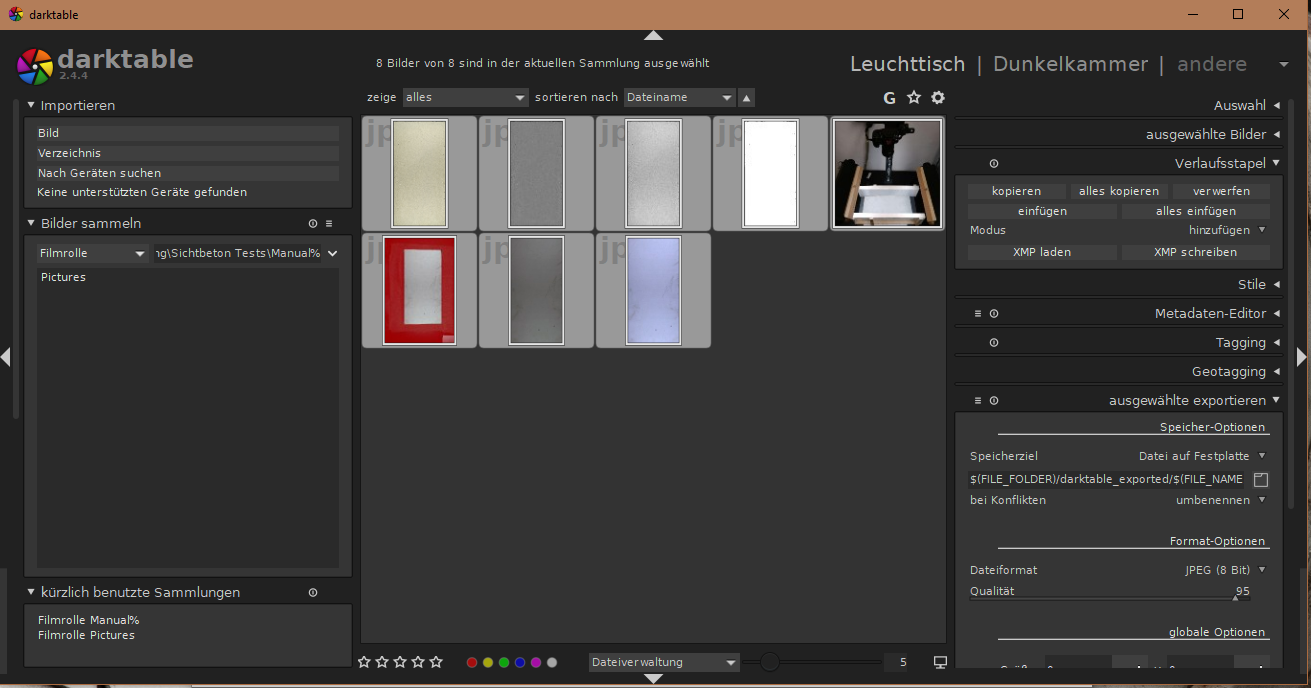
\includegraphics[width=\textwidth]{pictures/Darktable.png}
	\label{pic:darktable}
	\caption{Oberfläche von Darktable 2.4.4 im Bereich \textit{Leuchttisch}}
\end{figure}

\subsection{Auswertung}

Zur Auswertung müssen alle Bilder einer Serie in einem Ordner liegen. Anschließend wird das Script \textit{start\_process.py} ausgeführt werden. Dieses Script fragt nach dem Ausführen nach dem Speicherort der zu analysierenden Bilder und startet im Anschluss ein \textsc{ImageJ} Makro, das die Bilder weiterverarbeitet und Messwerte erzeugt, die in CSV-Dateien abgespeichert werden.

Abschließend wertet das Pythonscript diese CSV-Daten automatisiert aus und erstellt im angegebenen Bildordner eine Datei Namens \textit{results$X$x$Y$.csv}, in der die Ergebnisse aller Bilder zusammengefasst wurden.

Details zu dem Prozess finden sich in Kapilel \ref{sec:Algorithmus}.


\section{Beispiele}
\subsection{Grenzen der Beleuchtungsfehlerkorrektur}

Das folgende Beispiel zeigt eine Sichtbetonoberfläche mit einer starken Fehlbelichtung durch einen Schlagschatten (Abb. \ref{pic:example1a}) im Vergleich zu einer weniger starken Fehlbeleuchtung derselben Oberfläche (Abb. \ref{pic:example2a}) sowie die Ergebnisse der automatischen Korrektur (Abb. \ref{pic:example1b} bzw. \ref{pic:example2b}). Es wird deutlich, dass die Korrektur bei zu scharfkantigen Schlagschatten den Beleuchtungsfehler nicht mehr vollständig ausgleichen kann, während weiche Helligkeitsverläufe entfernt werden. Dies sollte in der Auswertung berücksichtigung finden, falls der Probekörper eine inhomogene Helligkeit über die Fläche hat. Diese könnte duch diese Methode herausgerechnet werden und wird daher in der Auswertung nicht berücksichtigt.

\begin{figure}[htbp]
	\centering
	\subfigure[Starker Beleuchtungsfehler durch Schlagschatten]{
		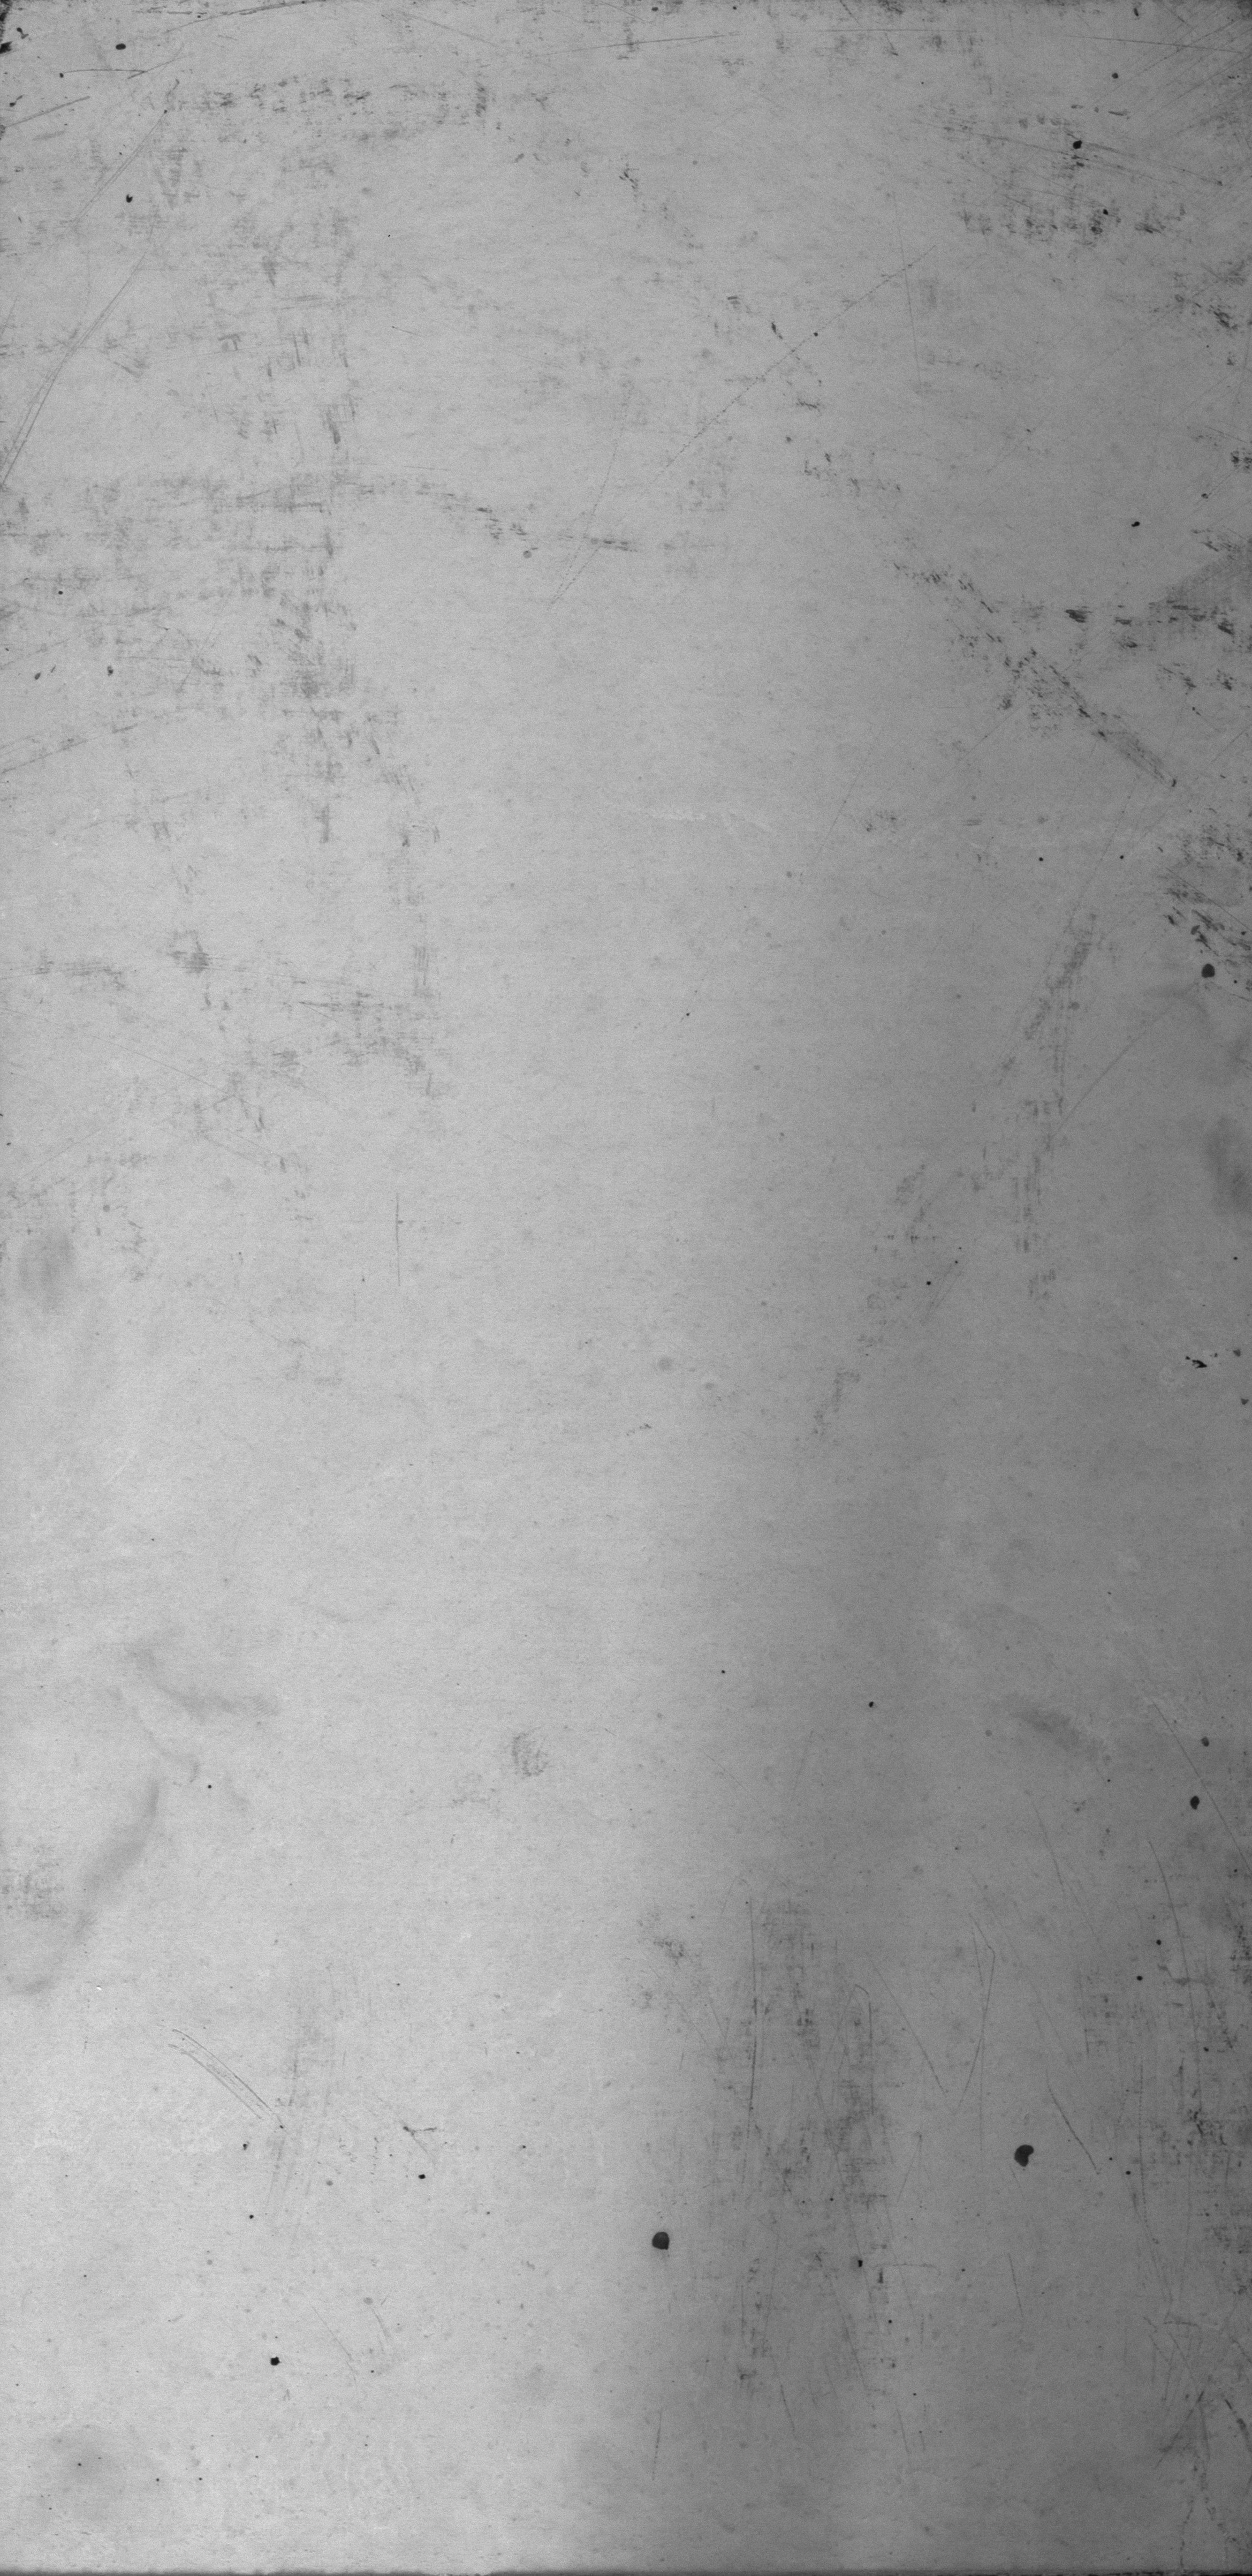
\includegraphics[width=0.2\textwidth]{pictures/example/1a_orig.jpg}
		\label{pic:example1a}
	}
	\subfigure[Korrigiertes Bild mit Fehlern]{
		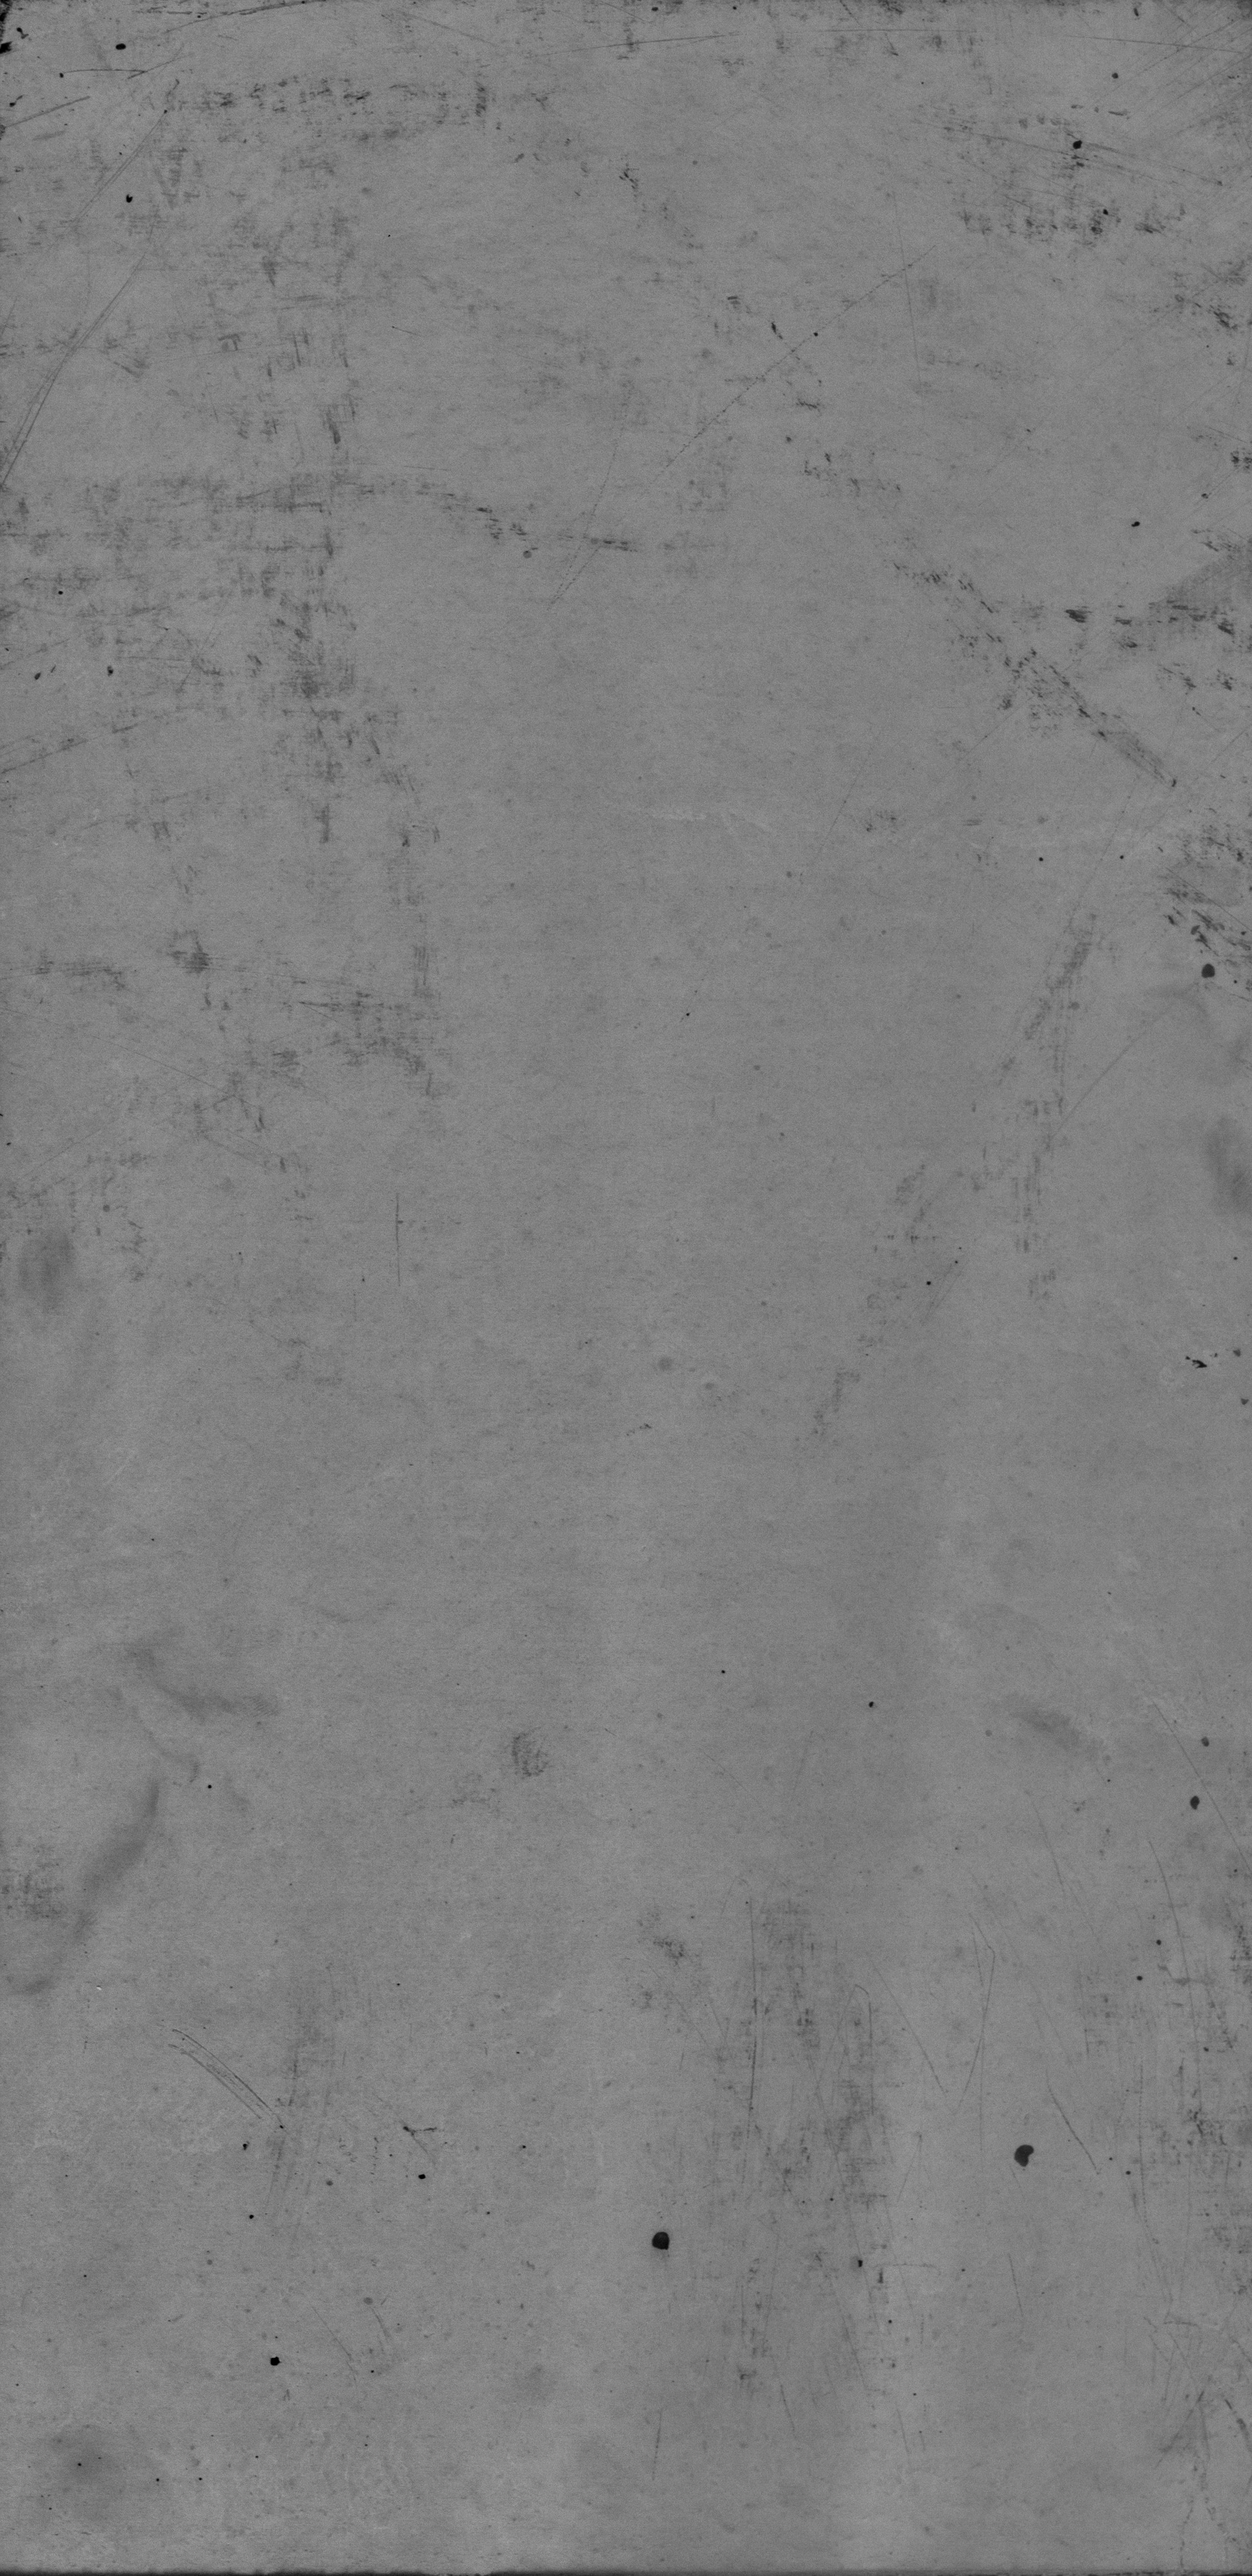
\includegraphics[width=0.2\textwidth]{pictures/example/1a_corr.jpg}
		\label{pic:example1b}
	}
	\subfigure[Leichter Beleuchtungsfehler]{
		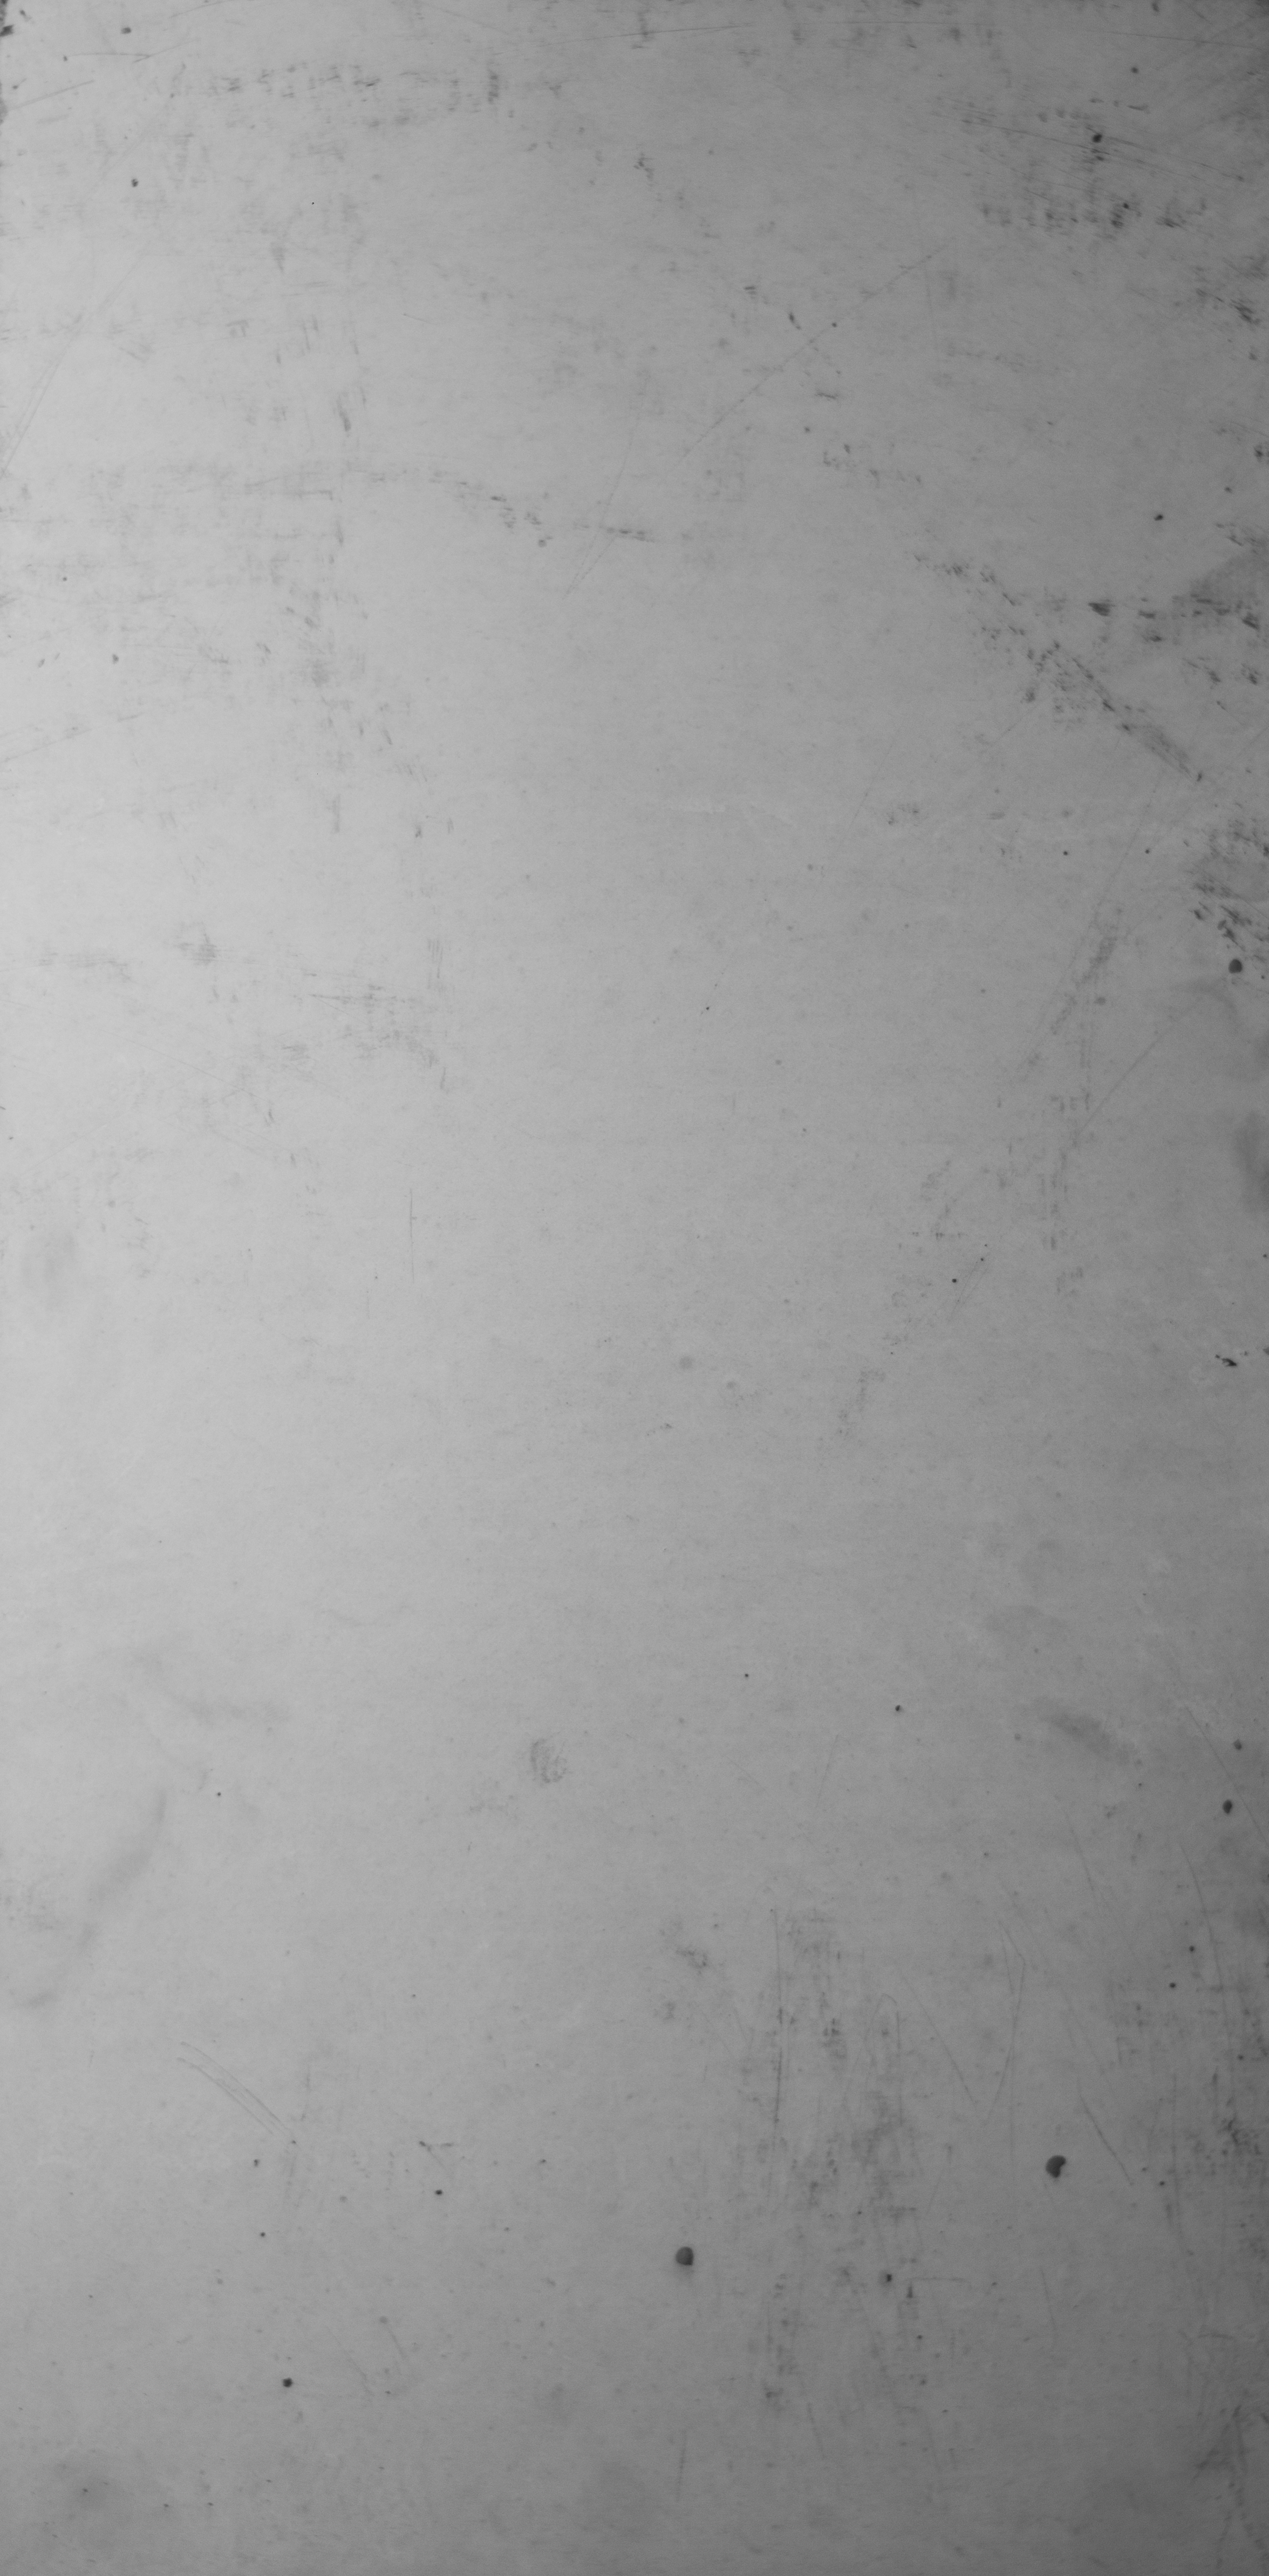
\includegraphics[width=0.2\textwidth]{pictures/example/1b_orig.jpg}
		\label{pic:example2a}
	}
	\subfigure[Korrigiertes Bild]{
		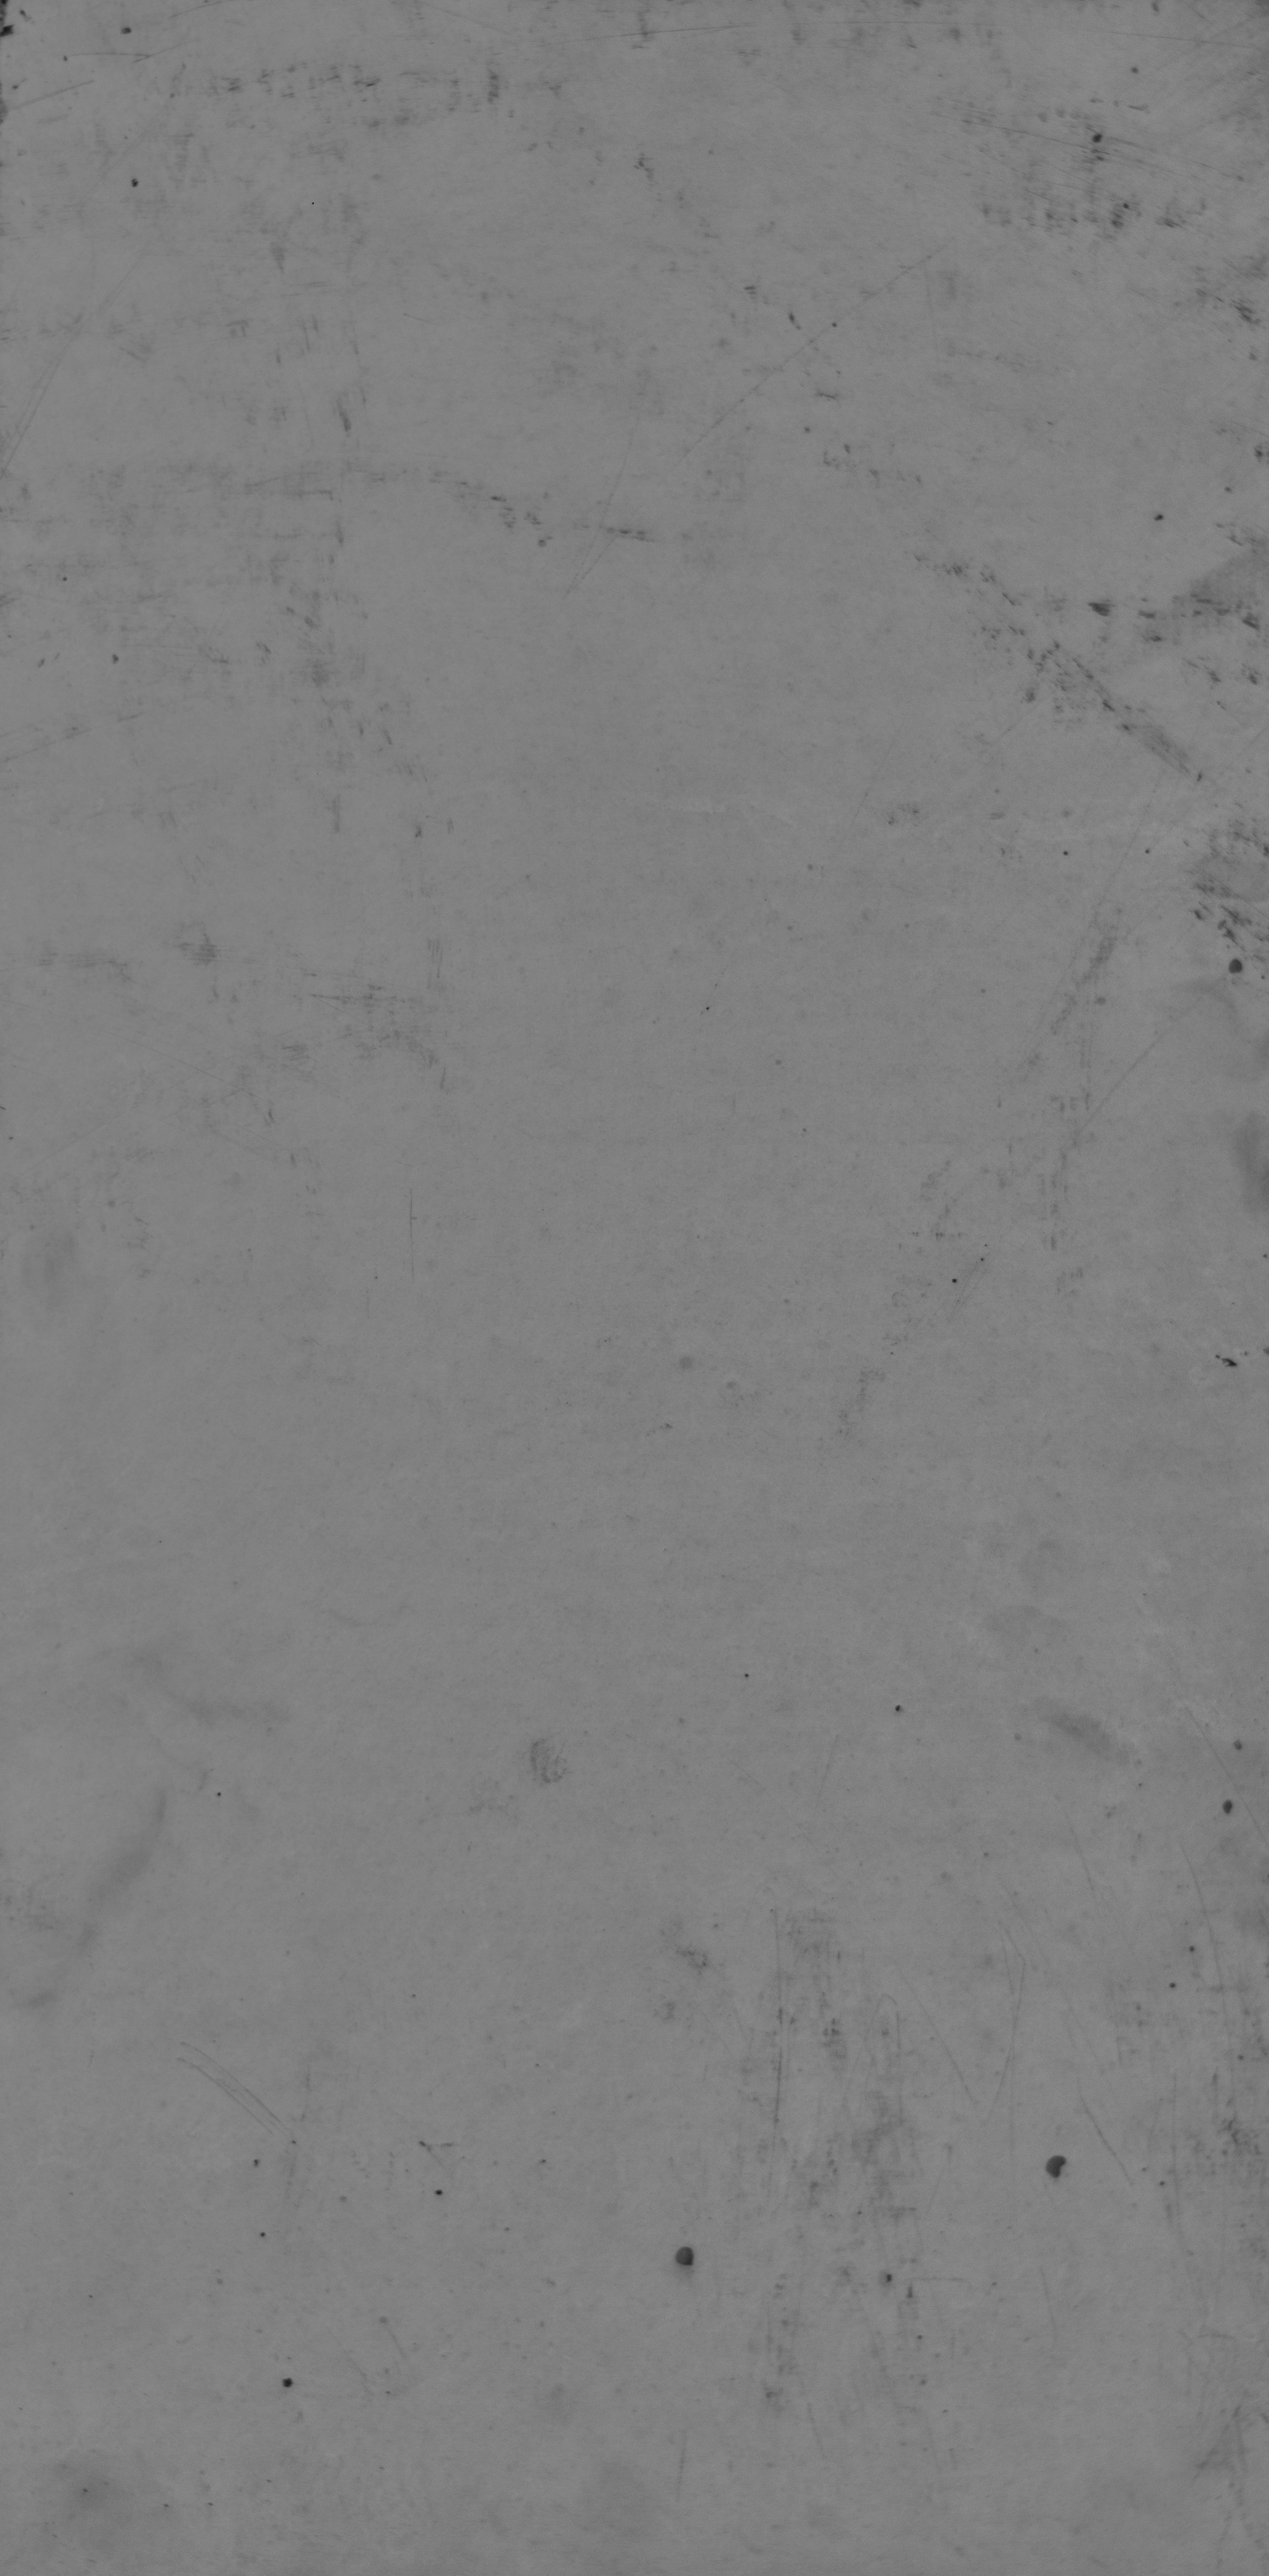
\includegraphics[width=0.2\textwidth]{pictures/example/1b_corr.jpg}
		\label{pic:example2b}
	}
	\caption{Einfluss der Art der Beleuchtungsfehler auf die Bildkorrektur}
\end{figure}

\subsection{Vergleich unterschiedlicher Sichtbetonoberflächenqualitäten}

Anhand der folgenden Proben werden beispielhaft die Ergebnisse des Scriptes ausgewertet. Die Unterteilungsparameter wurden wie folgt gewählt: $X = 4$ und $Y = 8$. 

\begin{figure}[htbp]
	\centering
	\subfigure[A: Inhomogene Oberfläche]{
		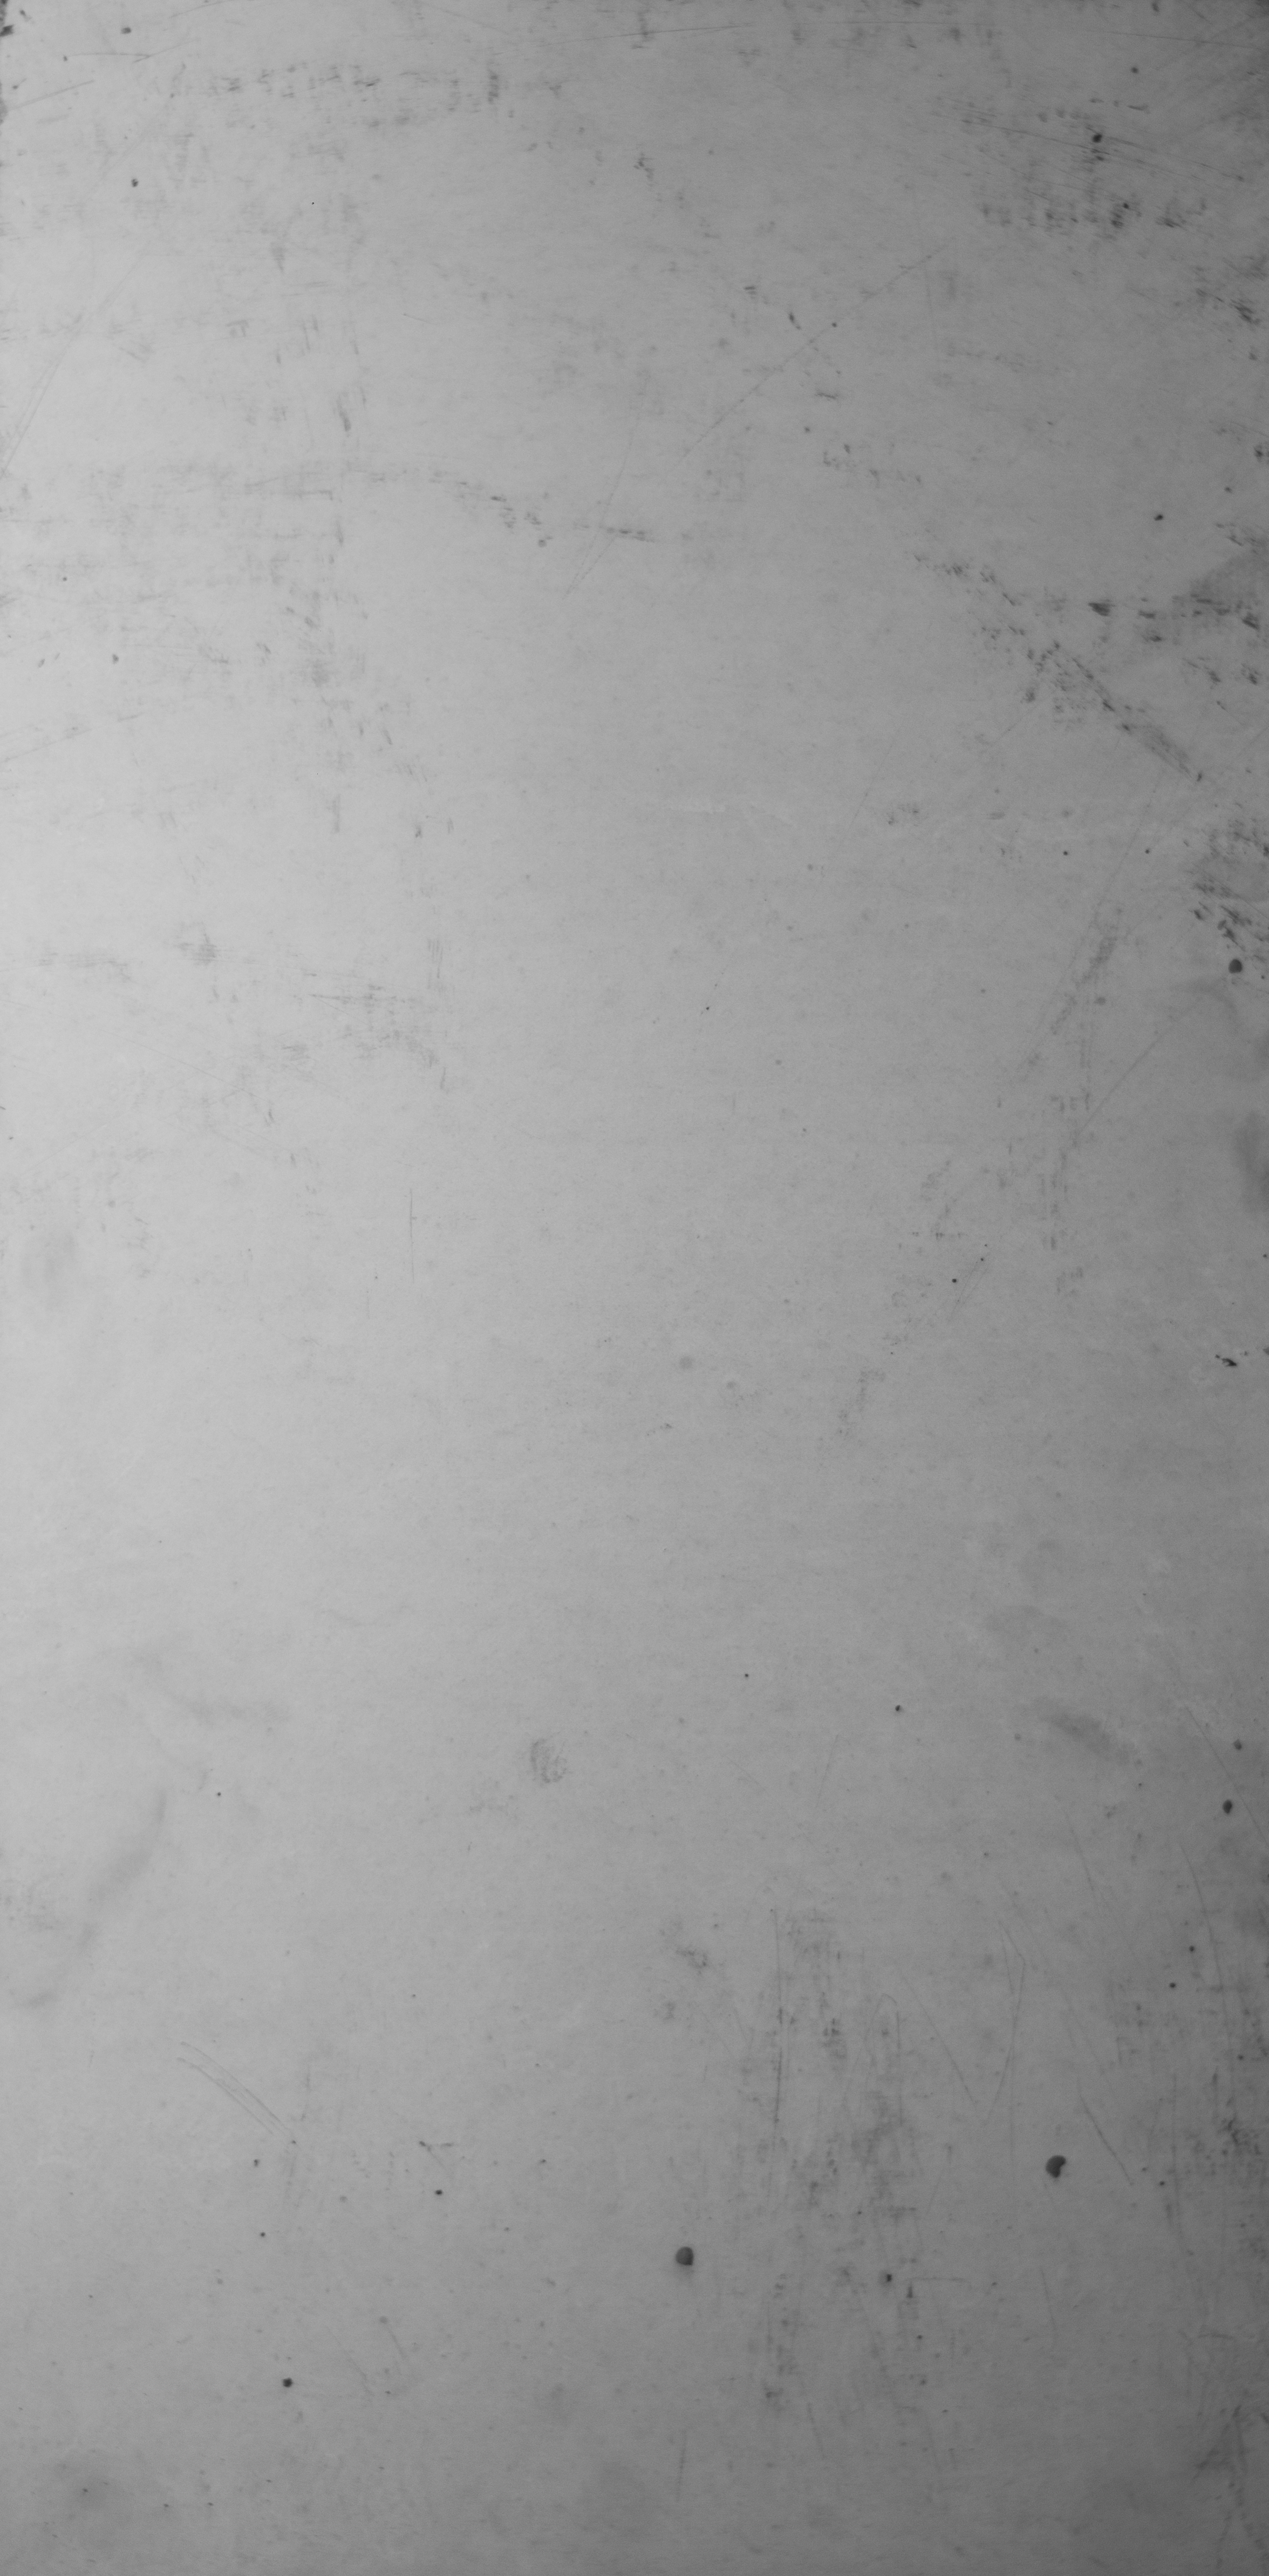
\includegraphics[width=0.31\textwidth]{pictures/example/1b_orig.jpg}
		\label{pic:example3a}
	}
	\subfigure[B: Inhomogene Oberfläche]{
		\includegraphics[width=0.31\textwidth]{pictures/example/4a_orig.jpg}
		\label{pic:example4a}
	}
	\subfigure[C: Homogene Oberfläche]{
		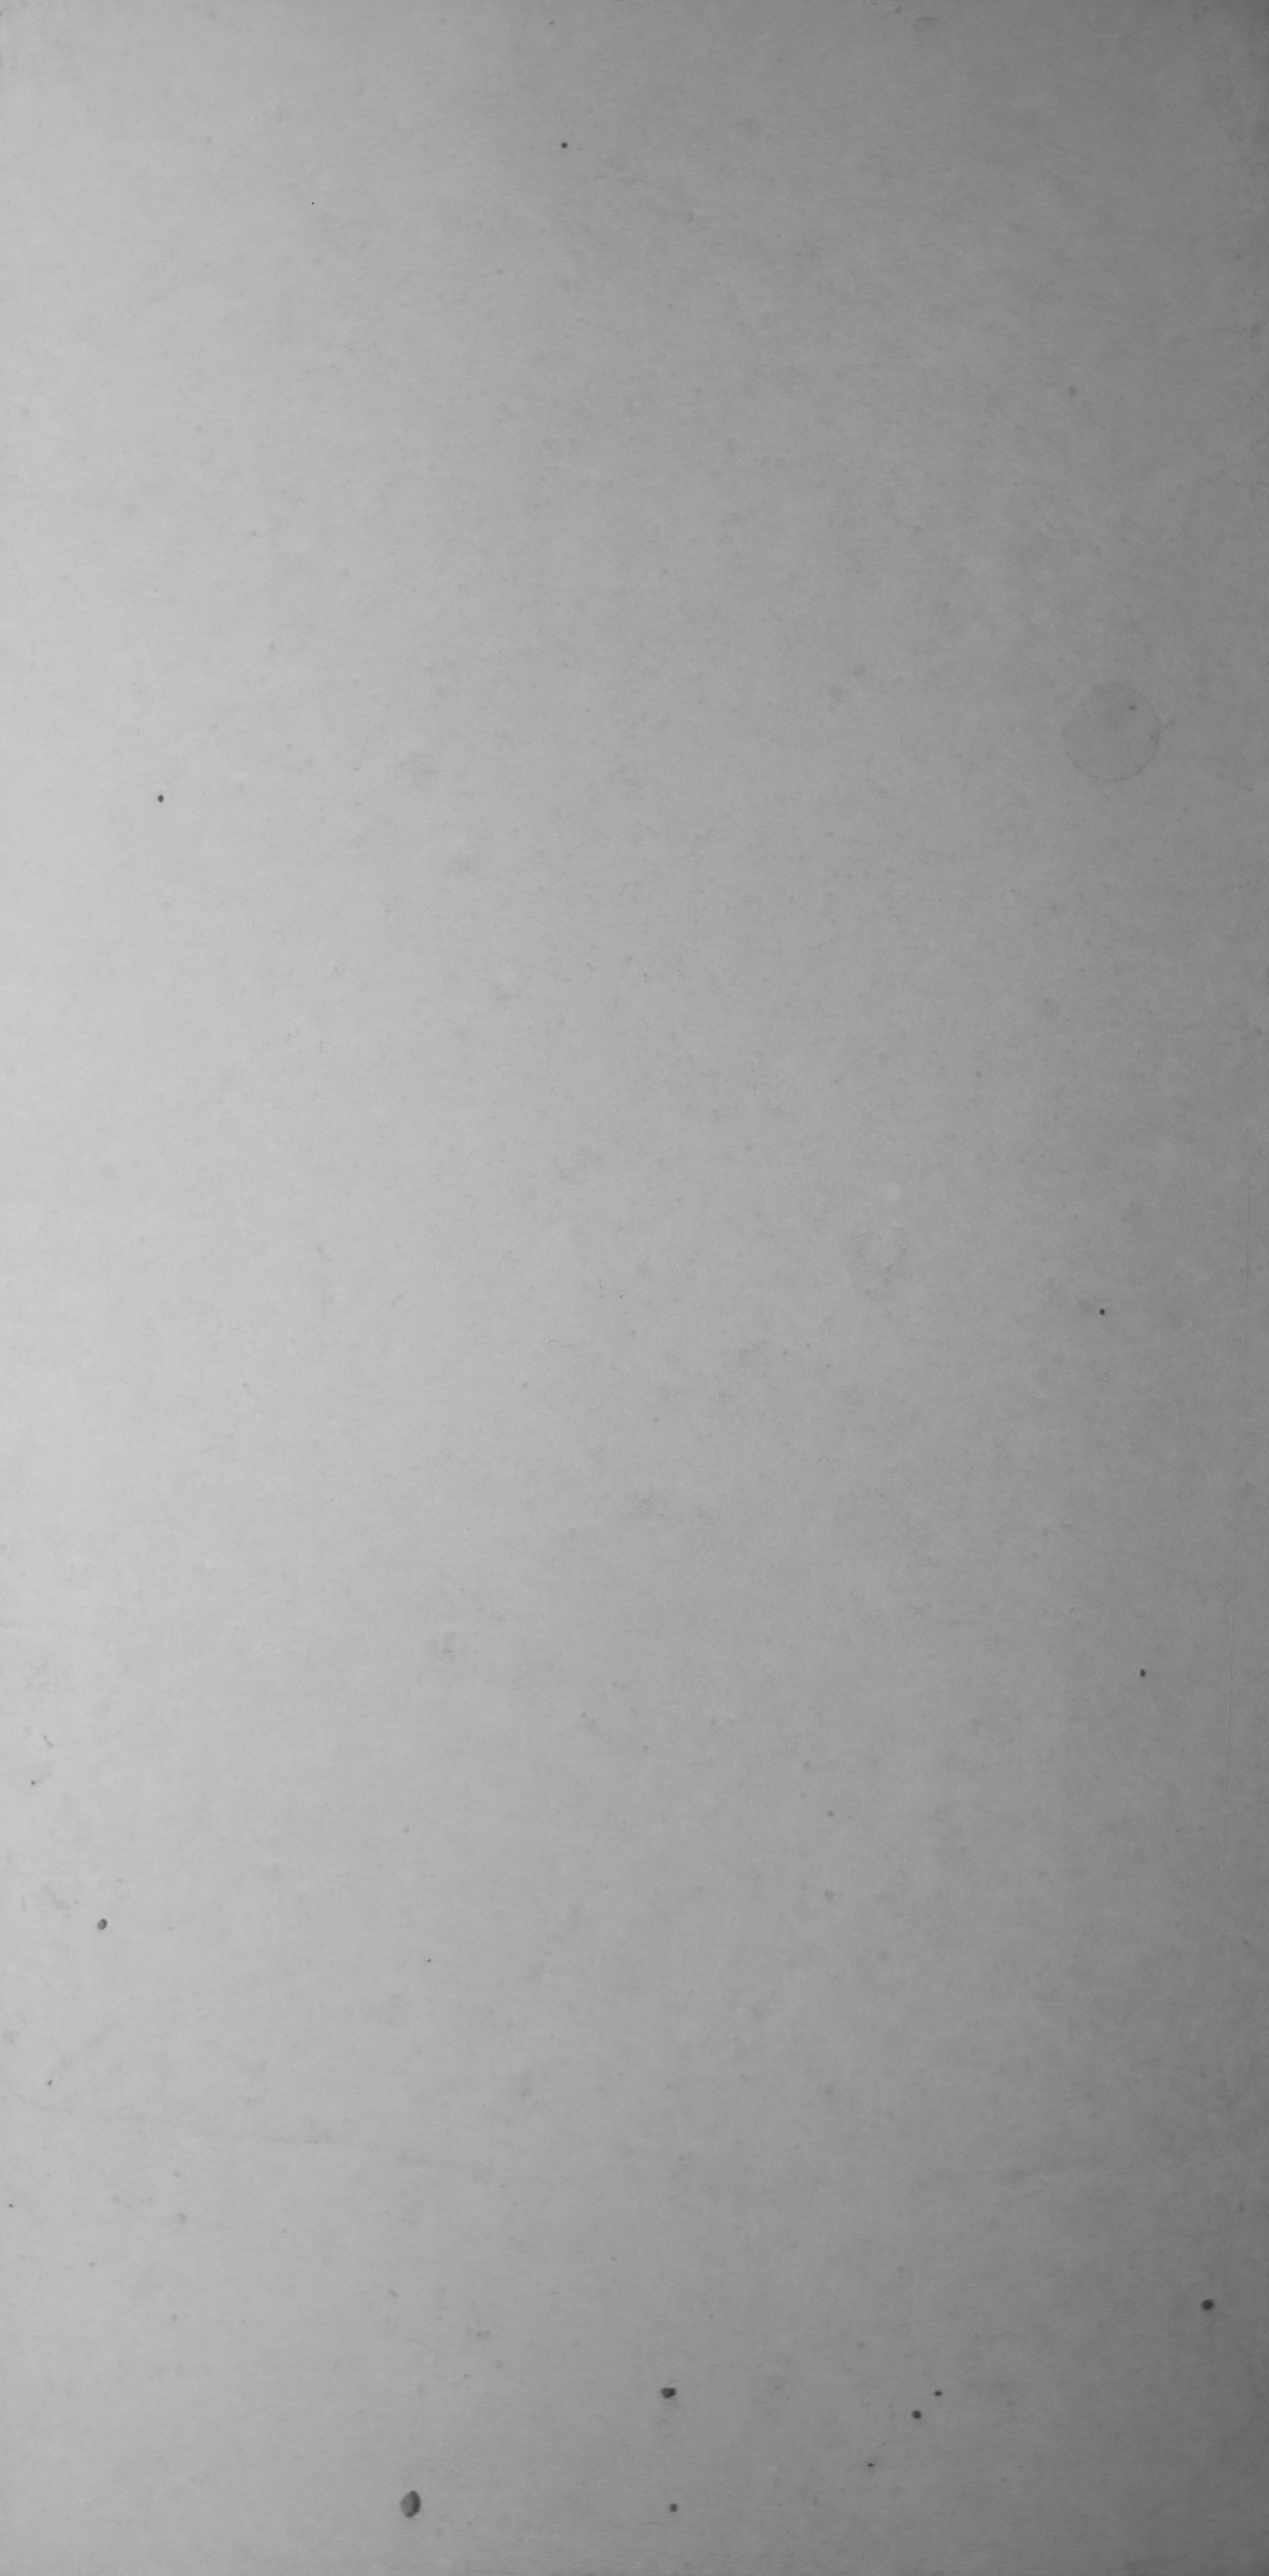
\includegraphics[width=0.31\textwidth]{pictures/example/3a_orig.jpg}
		\label{pic:example5a}
	}
	\caption{Verschiedene Sichtbetonqualitäten}
\end{figure}

Die Werte $\bar{\sigma}$, $\delta N$ und $\delta N_\text{max}$ in Tabelle \ref{tab:ergebnisse} beziehen sich auf die Abweichung des Farbwertes (zwischen 0 und 255), während die Poren in \% angegeben sind.

\begin{table}[ht]
	\centering
	\caption{Ergebnisse drei verschiedener Proben}
	\begin{tabular}{lcccc}
		\toprule
		Probe & $\bar{\sigma}$ & $\delta N$ & $\delta N_\text{max}$ & Poren\\
		\midrule
		A & 4,157 & 0,554 & 1,378 & 0,0058 \% \\
		B & 4,455 & 0,434 & 1,327 & 0,0041 \% \\
		C & 3,002 & 0,391 & 1,243 & 0,0043 \% \\
		\bottomrule
	\end{tabular}
	\label{tab:ergebnisse}
\end{table}

$\bar{\sigma}$ bezieht sich auf die durchschnittliche Farbabweichung innerhalb der Bereiche, $\delta N$ auf die Farbunterschiede benachbarter Bereiche und $\delta N_\text{max}$ auf die höchste Abweichung dieser benachbarten Bereiche. Es zeigen sich bei den ausgewählten Proben dabei deutliche Unterschiede. Während Probe C hier immer die niedrigsten Werte aufweist, zeigt sich bei Probe A mit vielen inhomogen Verteilten Strukturen die höchsten $\delta N$ und $\delta N_\text{max}$-Werte. Die Abweichung innerhalb der einzelnen Sektoren $\bar{\sigma}$ war bei dieser Probe hingegen geringer als bei Probe B, bei der die Strukturen homogener über die Gesamtfläche verteilt sind.

Aus den Zahlen erschließt sich also eine Bewertung der Qualität abhängig von der Verteilung der inhomogenitäten über die Oberfläche und lässt damit Rückschlüsse auf den Eindruck der Oberfläche auf den Beobachter aus verschiedenen Entfernungen zu. So wirken die in Probe A sichtbaren strukturen aus der Ferne störender als die Strukturen der Probe B.

\end{document}
